\documentclass[11pt]{article}

\usepackage{float}
\usepackage{hyperref}
\usepackage{fullpage}
\usepackage{verbatim}
\usepackage{moreverb}
\usepackage{graphicx}
\usepackage{parskip}
\usepackage{amsmath}
\usepackage[toc,page]{appendix}

\usepackage{minted}
\let\verbatiminput=\verbatimtabinput
\def\verbatimtabsize{4\relax}

\begin{document}
\title{EE 241B HW1 Writeup}

\author{Vighnesh Iyer}
\date{}
\maketitle

\tableofcontents

\section{Models - MOSFET Characterization}

We are using a 32nm LP CMOS process for this class. The devices being characterized are \verb|n105| and \verb|p105| (TT corner) with a nominal supply voltage of 1.05V.

\subsection{Threshold Voltages}
We want to determine the threshold voltage $V_{th}$ for the NMOS and PMOS devices (for $V_{BS}$ = 0, $L$ = 32nm, and $W$ = 1$\mu$m), by extrapolating from the $I_DS$ vs. $V_{GS}$ curve at low $V_{DS}$. We compare the threshold voltage derived from DC sweeps to the values reported in the model file and the DC operating point analysis.

To perform this characterization, we first collect a full range of DC operating points for both transistors to make analysis easier for this entire section. The transistors' drains are connected to a variable DC supply and the transistors' gates are connected to another independent variable DC supply. The source for both transistors is held at ground or VDD (0V/1.5V). We perform a nested DC analysis by sweeping $V_{DS}$ from $0 \rightarrow 1.05$V in (10mV) increments, and sweep $V_{GS}$ from $0 \rightarrow 1.05$V in (10mV) increments.

The gathered I-V curves are shown below.

\begin{figure}[H]
	\centerline{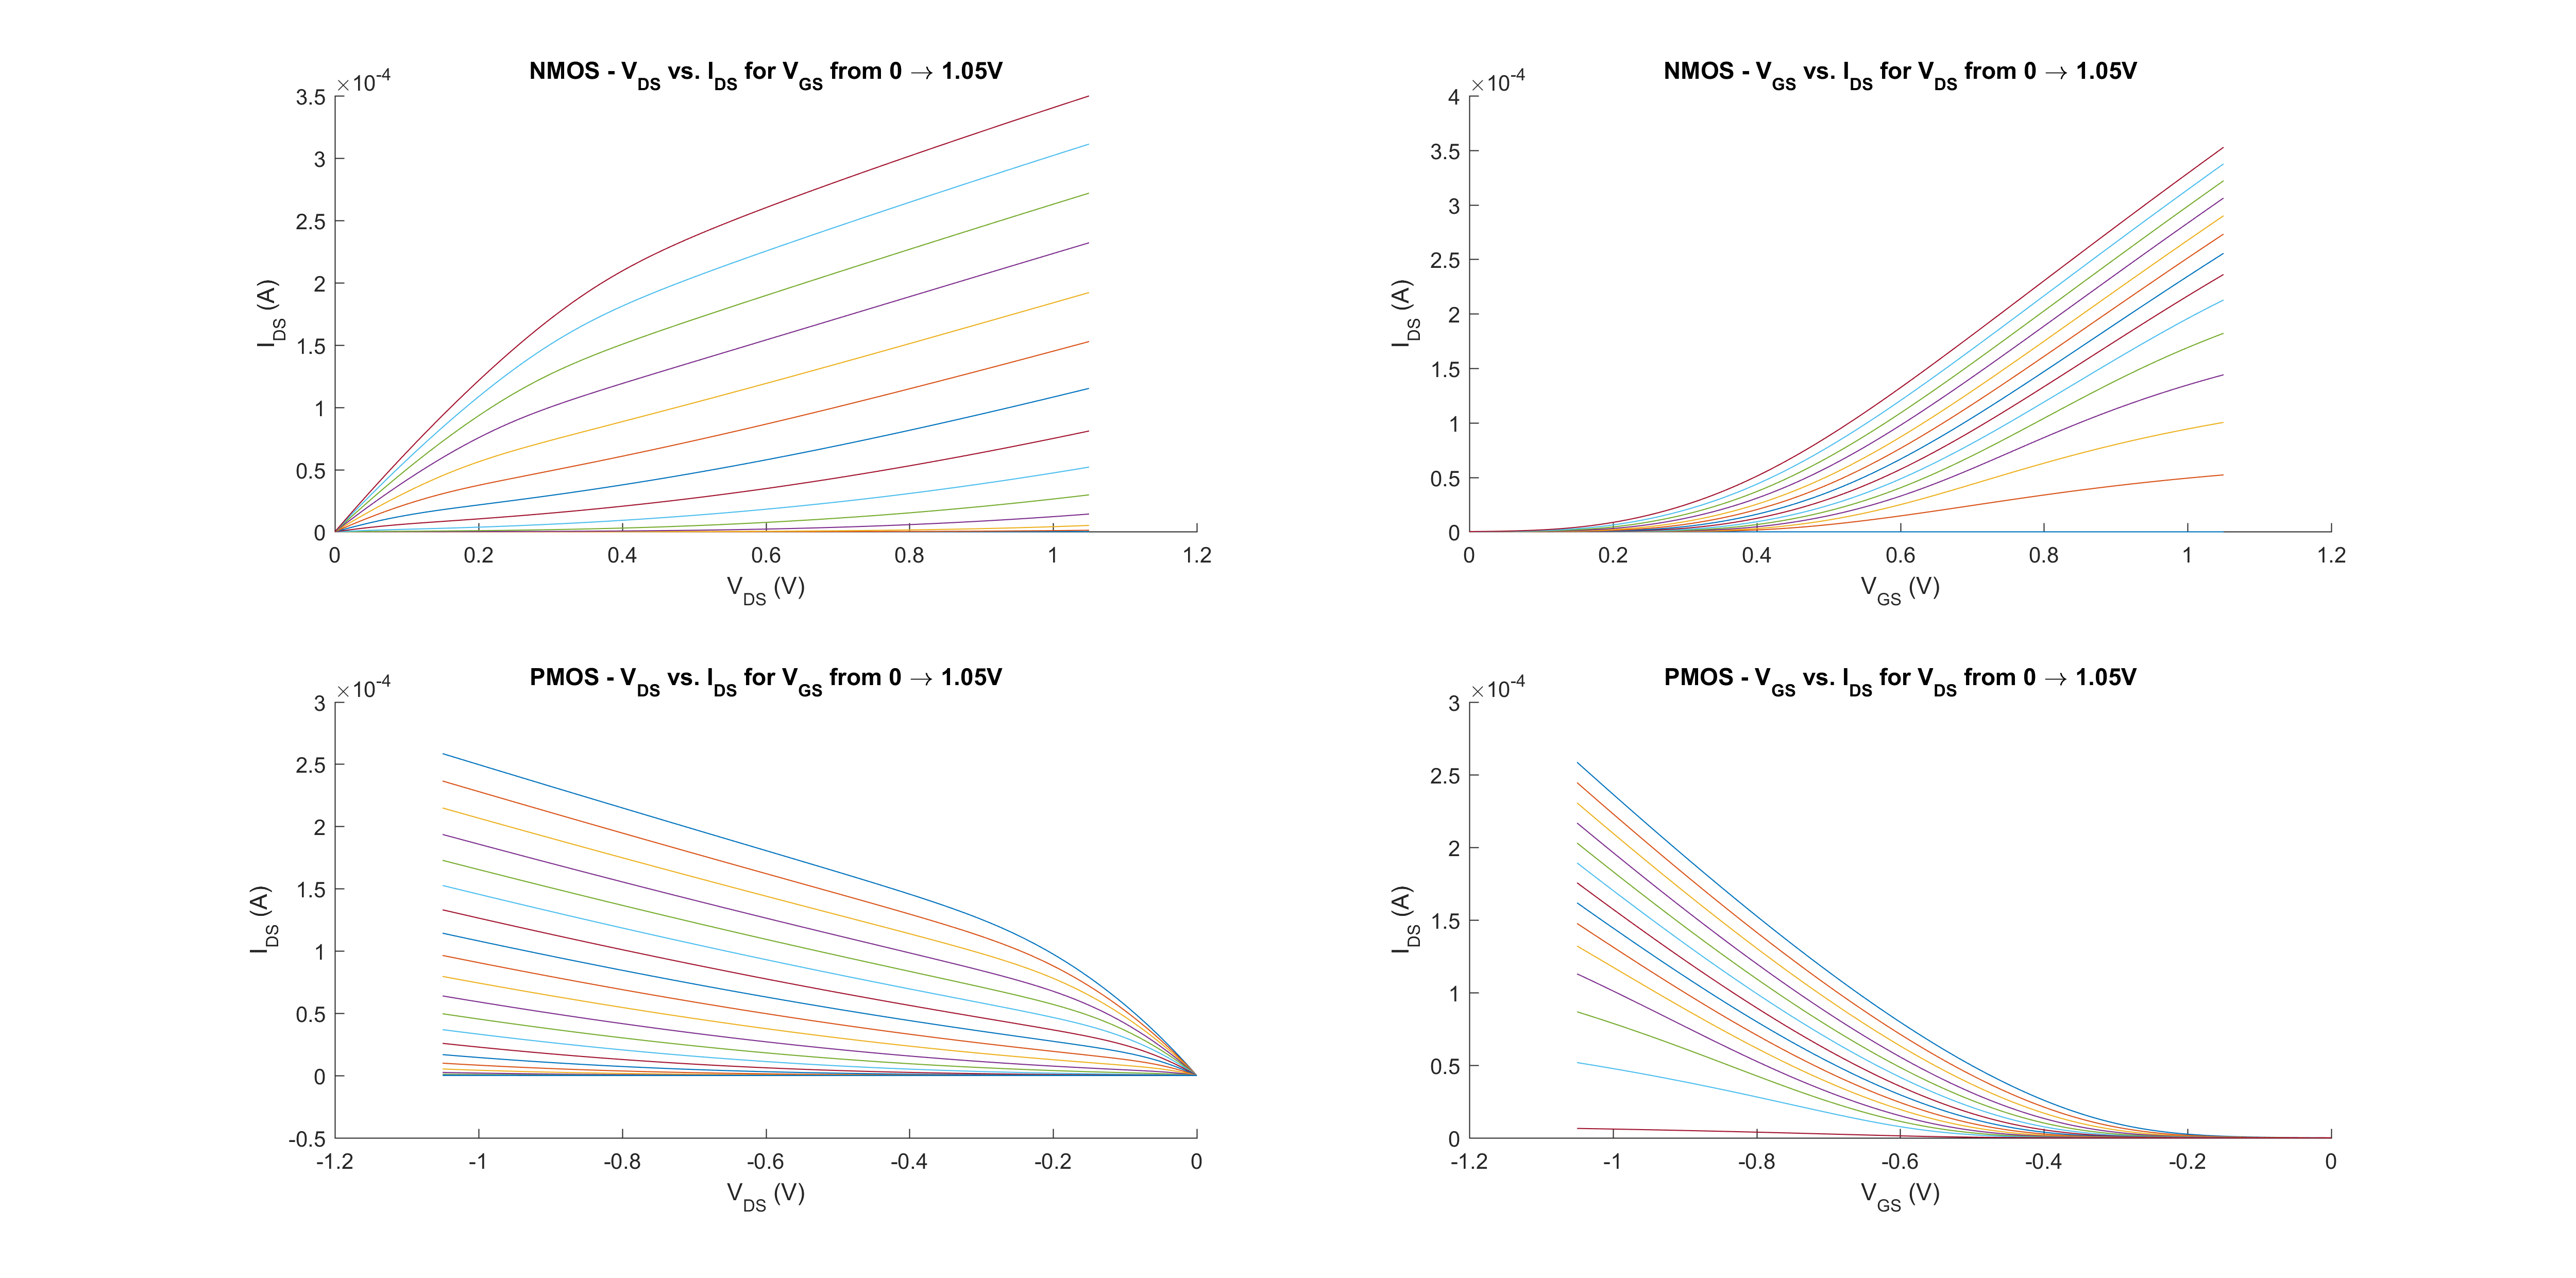
\includegraphics[width=\textwidth+5cm]{images/dc_curves.png}}	
\end{figure}

From the DC OP analysis, $V_{th}$ of the NMOS is reported to be 324.4 mV, and the $V_{th}$ of the PMOS is reported to be -208.1 mV. From the model files the NMOS $V_{th0}$ is 370 mV, and the PMOS $V_{th0}$ is -213 mV. However $V_{th0}$ is specified for long-channel devices, which don't accurately model the devices in this process.

To extract the threshold voltage from the I-V curves, we extrapolate the $V_{GS}$ vs $I_{DS}$ curves for a low value of $V_{DS}$ to keep the transistor in the linear region of operation. Then we fit a line to the linear part of the curves. We treat the x-intercept of those lines as the $V_{th}$ of the transistor for the selected value of $V_{DS}$. This method is shown for NMOS and PMOS transistors.

\begin{figure}[H]
	\centerline{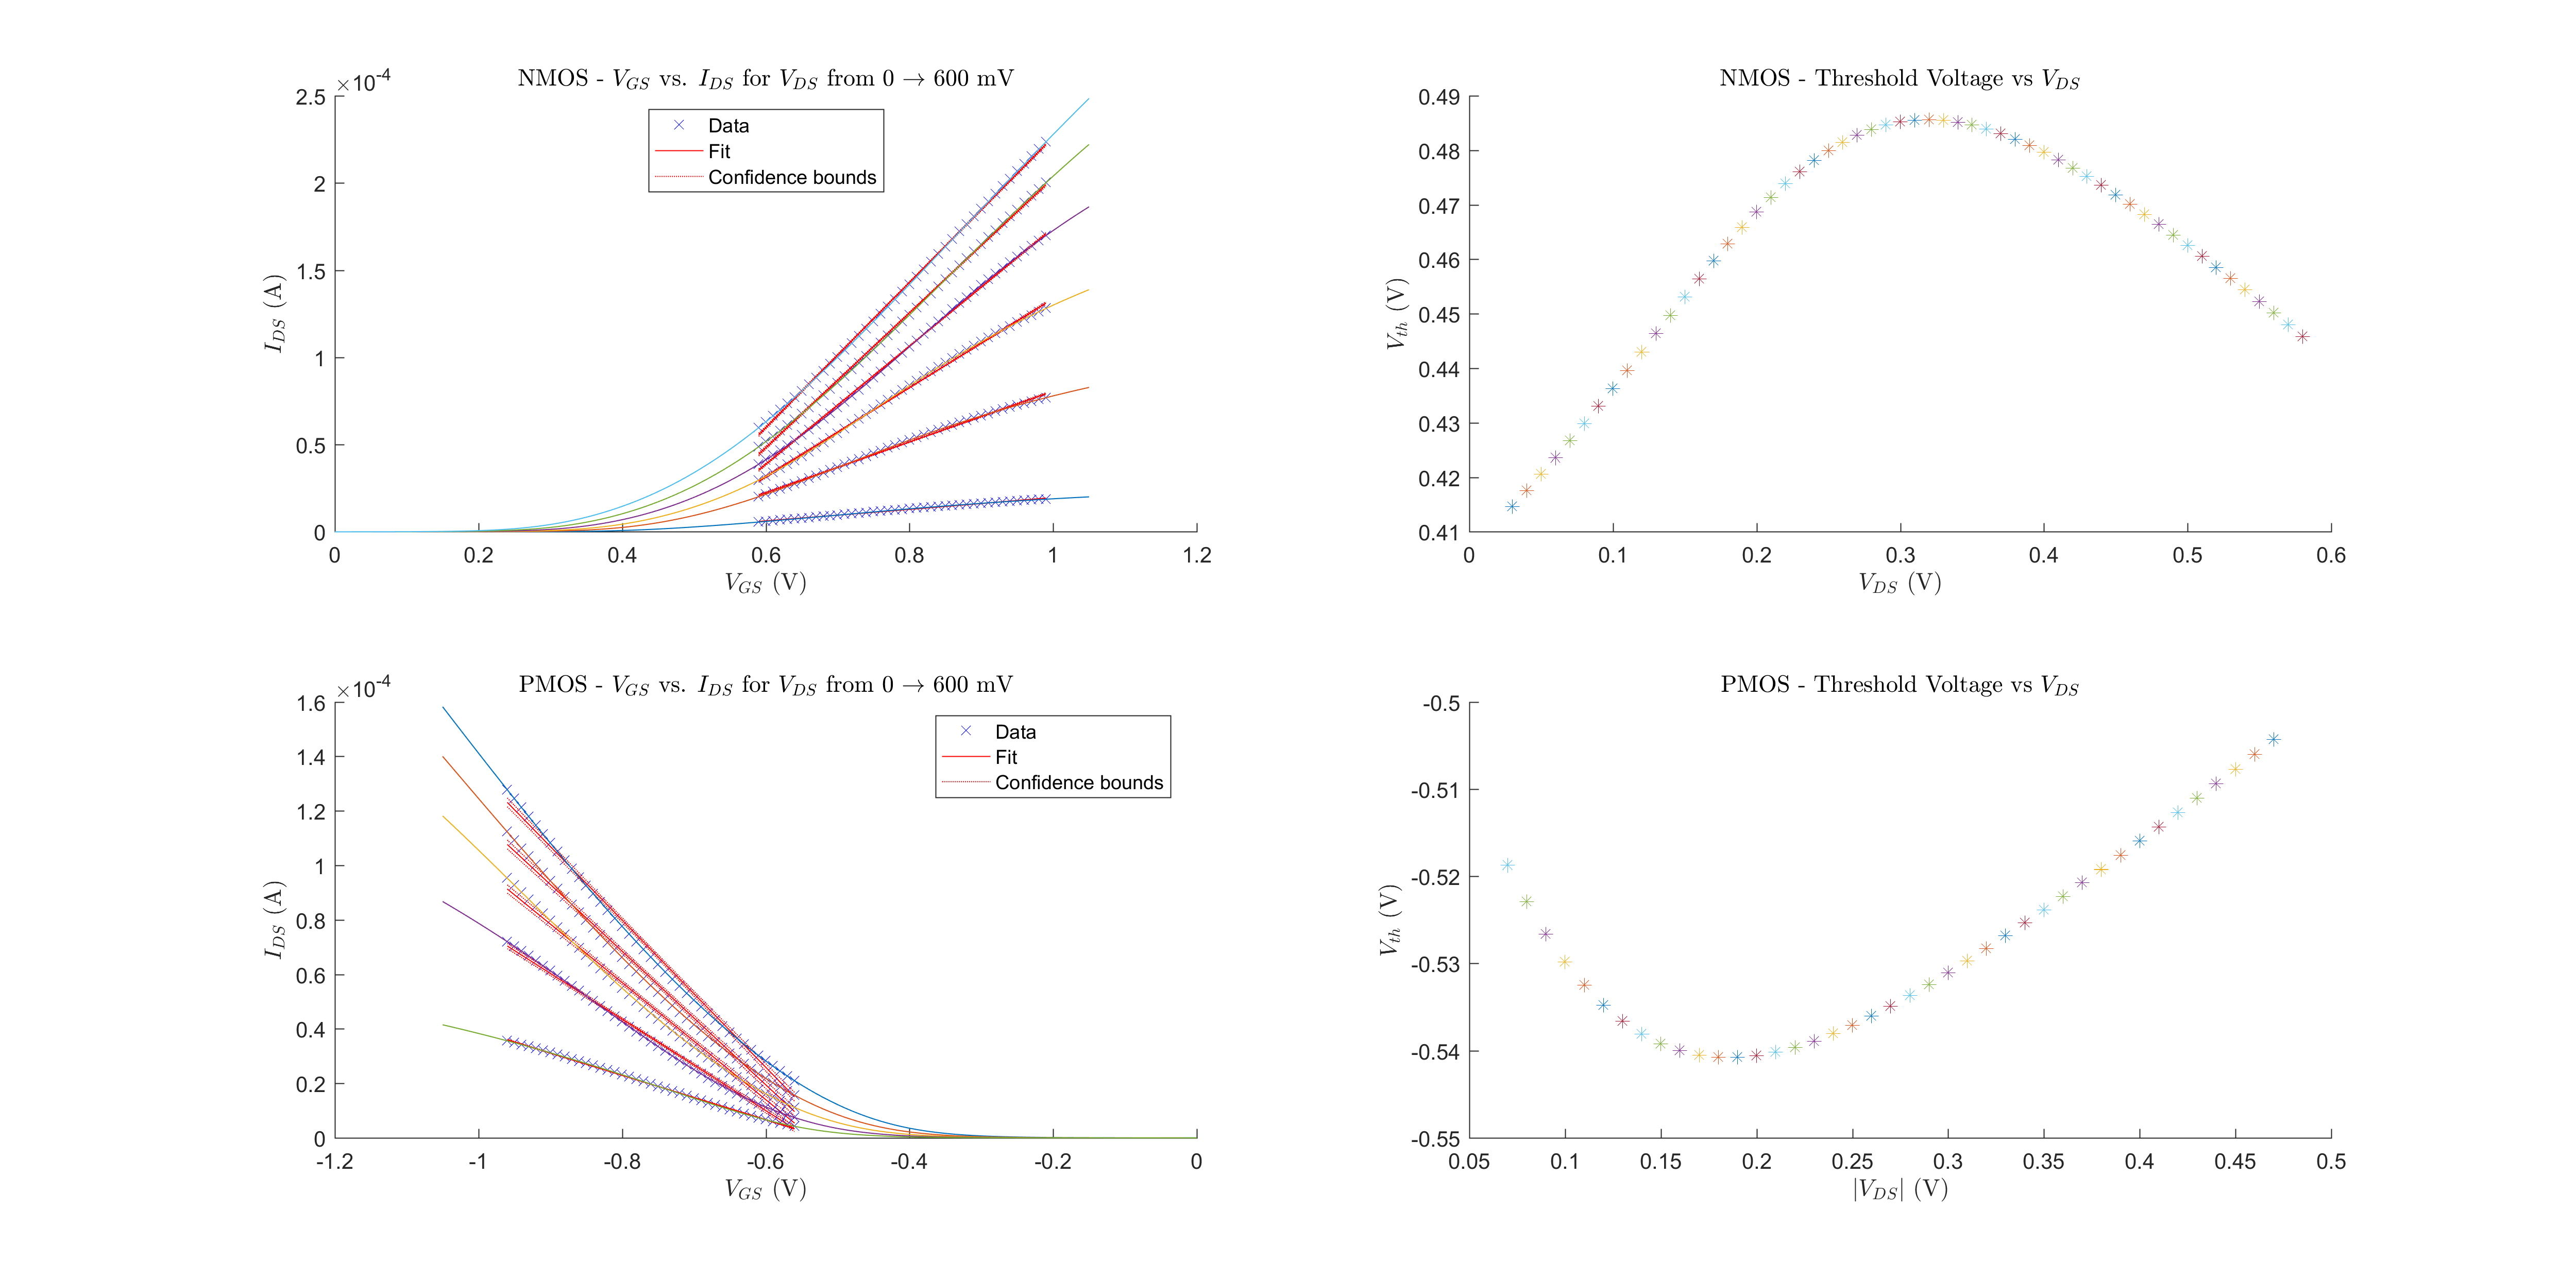
\includegraphics[width=\textwidth+5cm]{images/threshold_voltage.png}}	
\end{figure}

The images on the left side show the linear fit to each curve, while the images on the right side show the extrapolated $V_{th}$ for each $V_{DS}$ curve. As expected, with increased $V_{DS}$ the threshold voltage improves for both devices. 

The extrapolated results for the NMOS match the model files and the DC operating point measurement well. However, the PMOS threshold voltage is off by around 100 mV.

We can clearly see the effect of \textbf{DIBL} (drain induced barrier leakage) which is a result of voltage at the drain lowering the source potential barrier. This causes the $V_{th}$ to drop for higher values of $V_{DS}$. The initial 'increase' in $V_{th}$ for very low values of $V_{DS}$ is likely caused by the slightly worse linear fit that's used to extrapolate $V_{th}$.

\subsection{Fitting Velocity Saturation Model}
In class, we use this model for $I_{DSat}$:

\begin{equation*}
	I_{DSat} = \frac{W}{L} \frac{\mu_{eff} C_{ox} E_C L}{2} \frac{(V_{GS} - V_{th})^2}{(V_{GS} - V_{th}) + E_C L}
\end{equation*}

We want to find the values of $E_C L$ that best fit the NMOS and PMOS I-V curves. We will use the $V_{th}$ value from the previous section. We take the case of the $V_{DS}$ curve where $V_{DS} = V_{DD}$ to keep the transistors fully saturated and we sweep $V_{GS}$. We then fit out data where $V_{GS} > V_{th}$ to this model with $E_C L$ and $k = \mu_{eff} C_{ox}$ as free variables.

To get starting values for fit iteration, I used model parameters to estimate $k$. I found that for the NMOS $\mu_0$ (\verb|u0_n105|) is 30.4, $t_{ox}$ (\verb|toxe_n105|) is 2.39e-9, and $\epsilon_{ox}$ (\verb|epsrox|) is 3.9. For the PMOS $\mu_0$ (\verb|u0_p105|) is 60.95, $t_{ox}$ (\verb|toxe_p105|) is 2.62e-9, and $\epsilon_{ox}$ (\verb|epsrox|) is 3.9. We also know that $C_{ox} = \frac{\epsilon_{ox}}{t_{ox}}$.

Through experimentation, I found that $V_{th}$ from the previous section doesn't match this curve that well since the higher $V_{DS}$ results in a smaller effective threshold voltage. I then made $V_{th}$ another free variable to see if I could get a better fit.

After several iterations, it became clear that small changes in the initial guesses for the free variables resulted in very different curve fits. I settled on values that would give me a realistic $E_C L$ and $k$, but gave me a lower $V_{th}$ than expected.

\begin{figure}[H]
	\centerline{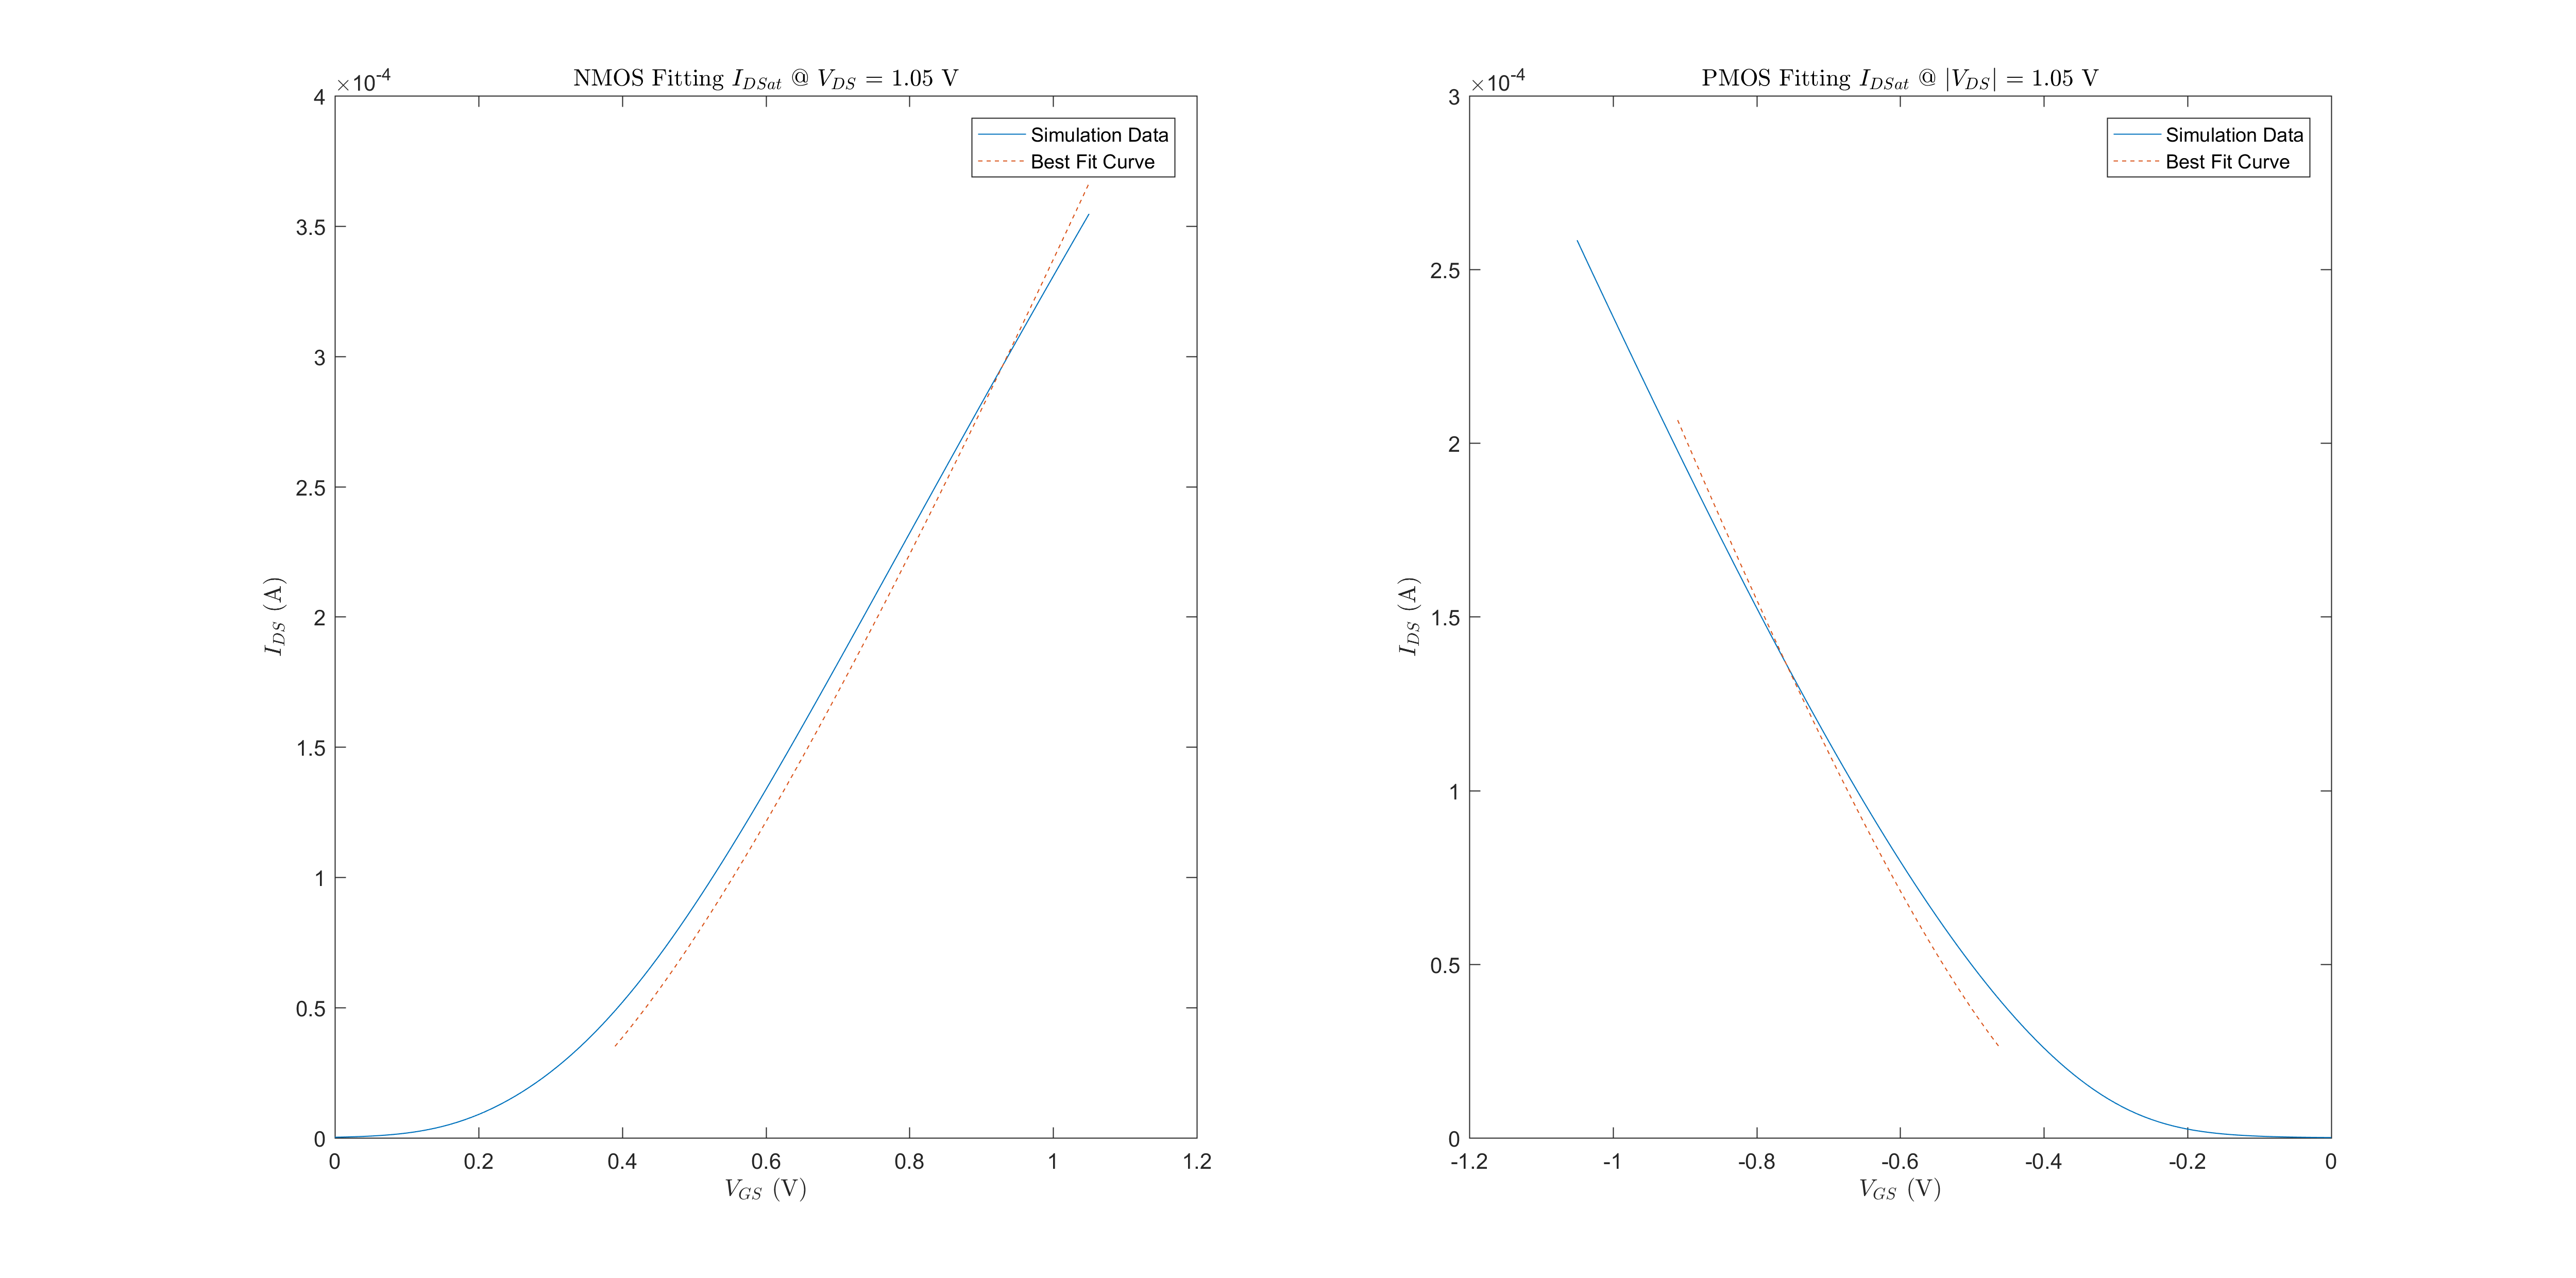
\includegraphics[width=\textwidth]{images/idsat_fit.png}}
\end{figure}

The NMOS fit gave free parameter values of $k = 0.0001, E_C L = 0.4859 \text{ V}, V_{th} = 0.2039 \text{ V}$. The PMOS fit gave values of $k = 0.0001, E_C L = 0.491 \text { V}, V_{th} = -0.2926 \text{ V}$. The threshold voltages are too low for this fit to be an accurate model. If I had additional time, I would have tried modifying the $I_{DSat}$ equation to take into account finite output resistance (FET Early Voltage), by adding a factor of $(1 + \lambda V_{DS})$ and treating $\lambda$ as another free parameter.

\subsection{Fitting Alpha-Power Law}
We now turn to the alpha-power-law model:

\begin{equation*}
	I_D = K(V_{GS} - V_{th}) ^ \alpha
\end{equation*}

This model is accurate when the transistor is in saturation and is presented by the paper "Alpha-Power Law MOSFET Model and its Applications to CMOS Inverter Delay and Other Formulas" by Sakurai and Newton. Using \verb|lsqcurvefit| in MATLAB, we determine the values of $K, V_{th}, \alpha$ that best fit the model.

\begin{figure}[H]
	\centerline{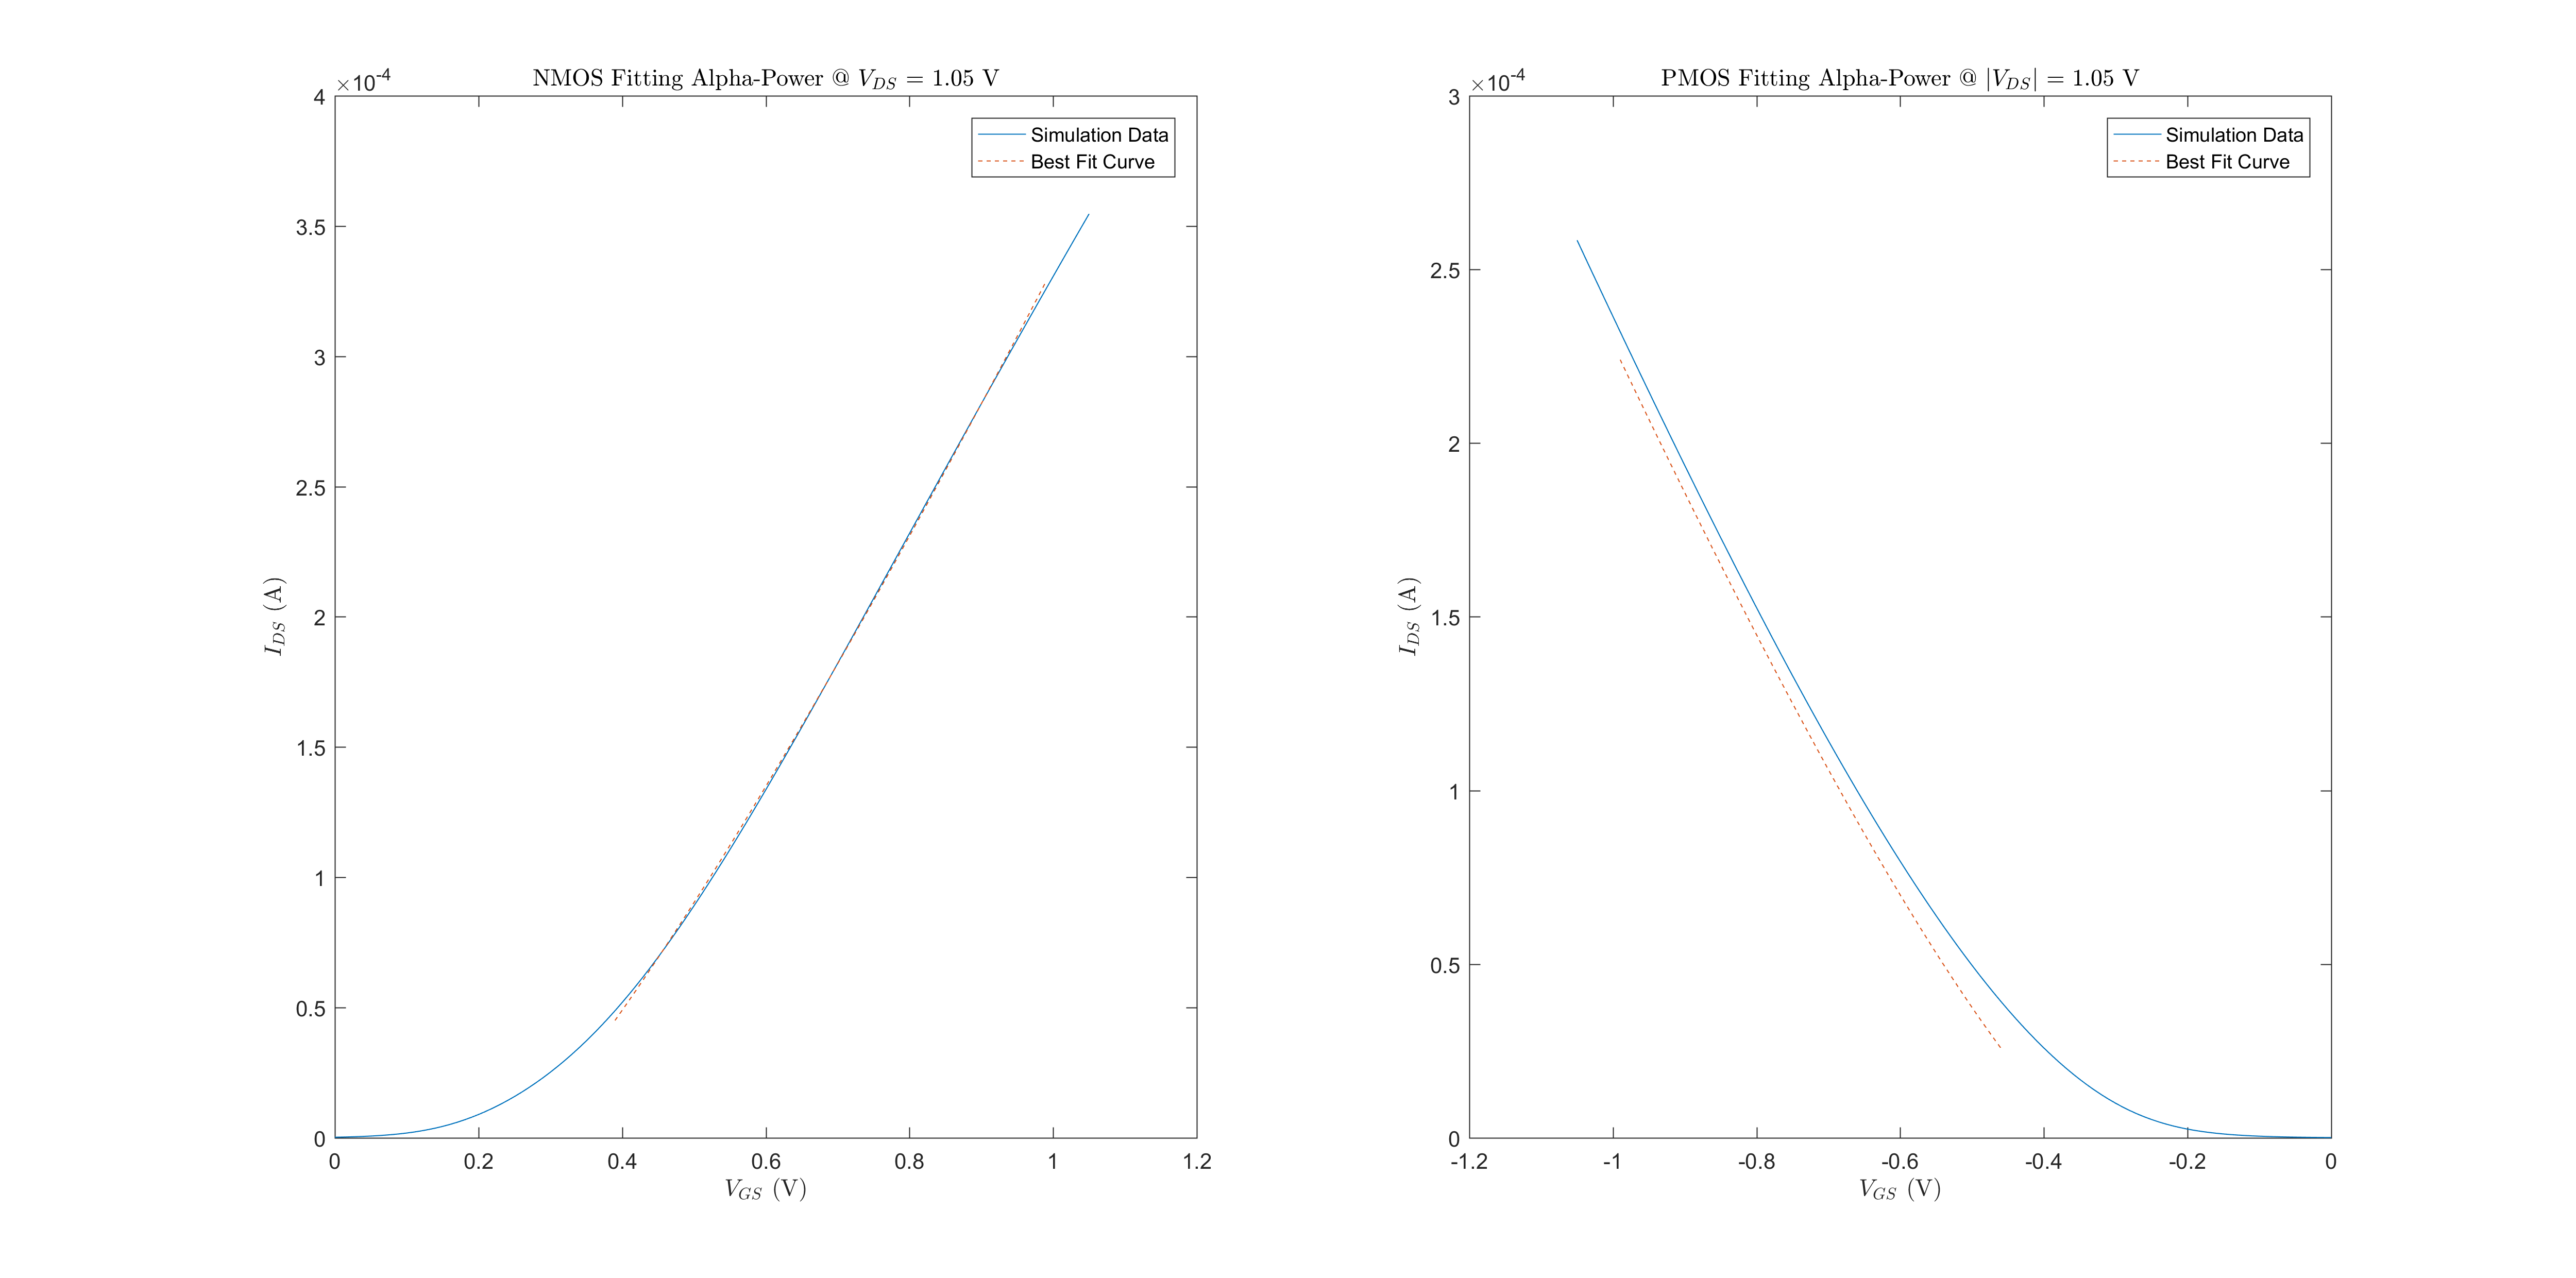
\includegraphics[width=\textwidth]{images/alpha_power_fit.png}}
\end{figure}

When fitting, I encountered the same issues from the previous section. Small variations in initial parameter estimates resulted in vastly different fits, and the final iteration produced a reasonable value for $K$ and $\alpha$, but gave a $V_{th}$ that was too low to be realistic.

For the NMOS, $\alpha = 1.183, K = 0.0005, V_{th} = 0.252 \text{ V}$, and for the PMOS $\alpha = 1.178, K = 0.0002, V_{th} = -0.382 \text{ V}$. 

\subsection{Fitting Alpha-Power Law ($\alpha = 1$)}
Now we fit the same alpha-power law model, but fix $\alpha$ to one to find the best $V_{th}$ that correspond to linear dependence of current on $V_{GS}$.

\begin{figure}[H]
	\centerline{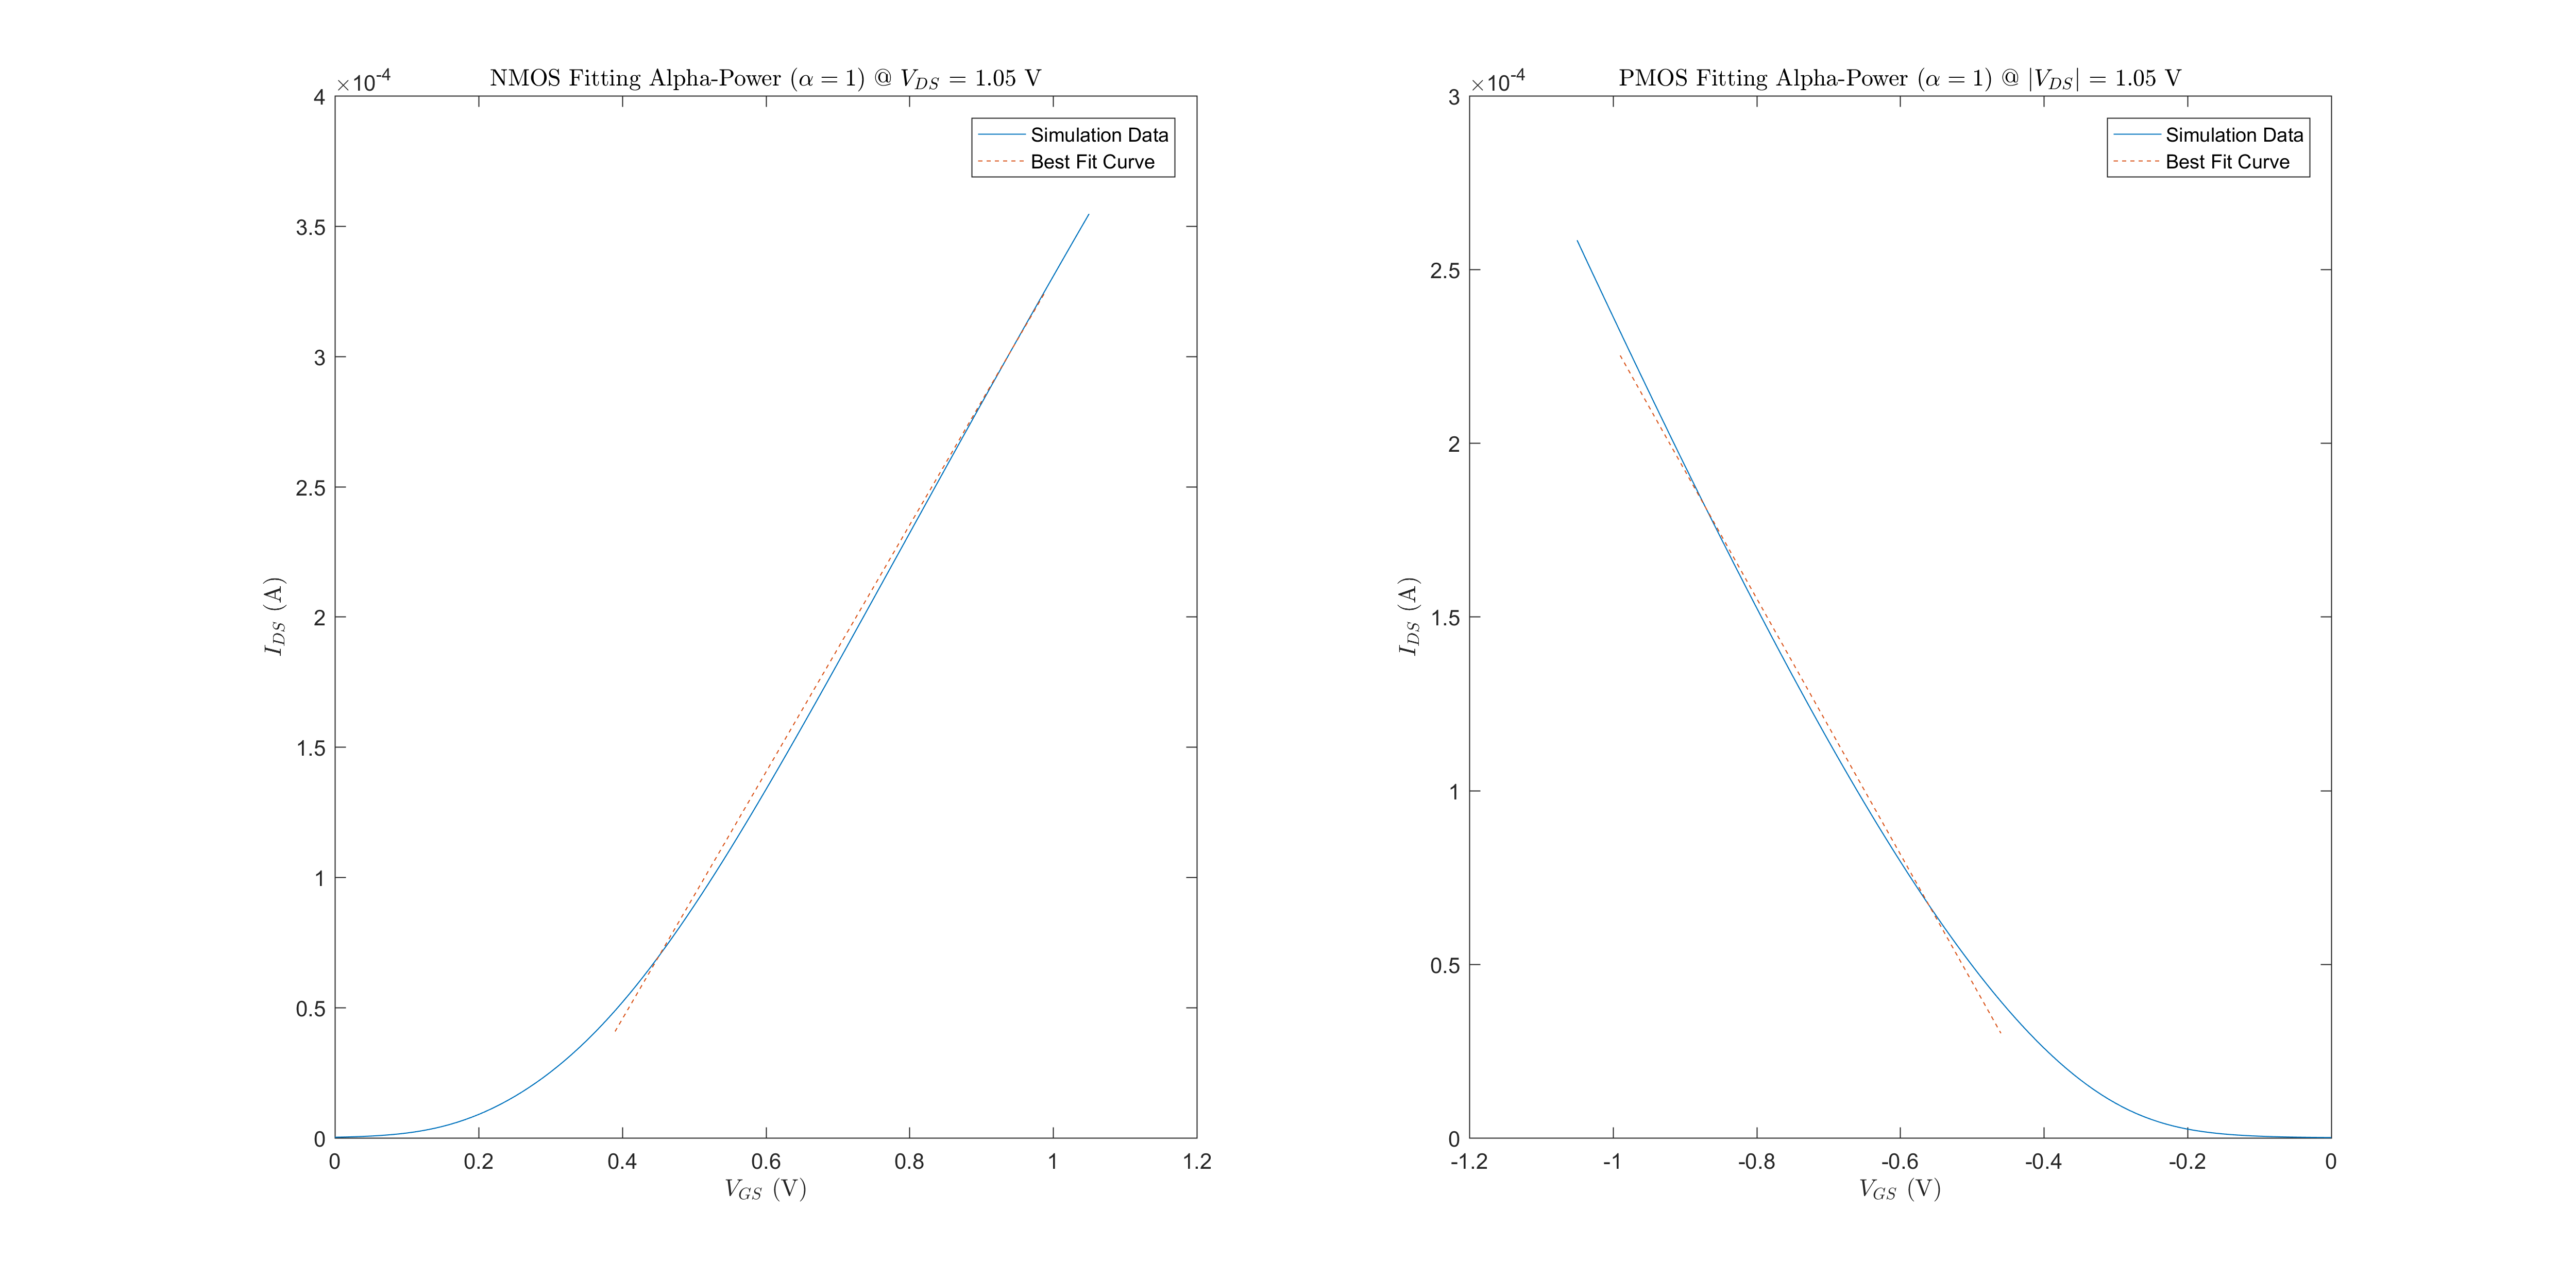
\includegraphics[width=\textwidth]{images/alpha_power_fit_alpha1.png}}
\end{figure}

These fits are fairly accurate when the transistor is deep in saturation. For the NMOS, $K = 0.0005, V_{th} = 0.3039 \text{ V}$, and for the PMOS, $K = 0.0004, V_{th} = -0.3782 \text{ V}$.

\section{Transistor Sizing}

\subsection{Find Ideal Ratio of PMOS/NMOS Widths for a CMOS Inverter}
Using SPICE and the 32nm LP model with a 1.05V supply, we find the optimal width of the PMOS transistor that minimizes the propagation delay ($t_{p} = (t_{pHL} + t_{pLH}) / 2)$ for a CMOS inverter. We fix the NMOS transistor width at 100nm and the lengths of both transistors are fixed at the process' 32nm minimum.

In order to solve this problem with simulation, I used the F04 (fanout of 4) method of inverter delay characterization. I designed a simulation based on the paper "The Fanout-of-4 Inverter Delay Metric" by Harris, Horowitz, et al. The circuit setup from the paper is shown below.

\begin{figure}[H]
	\centerline{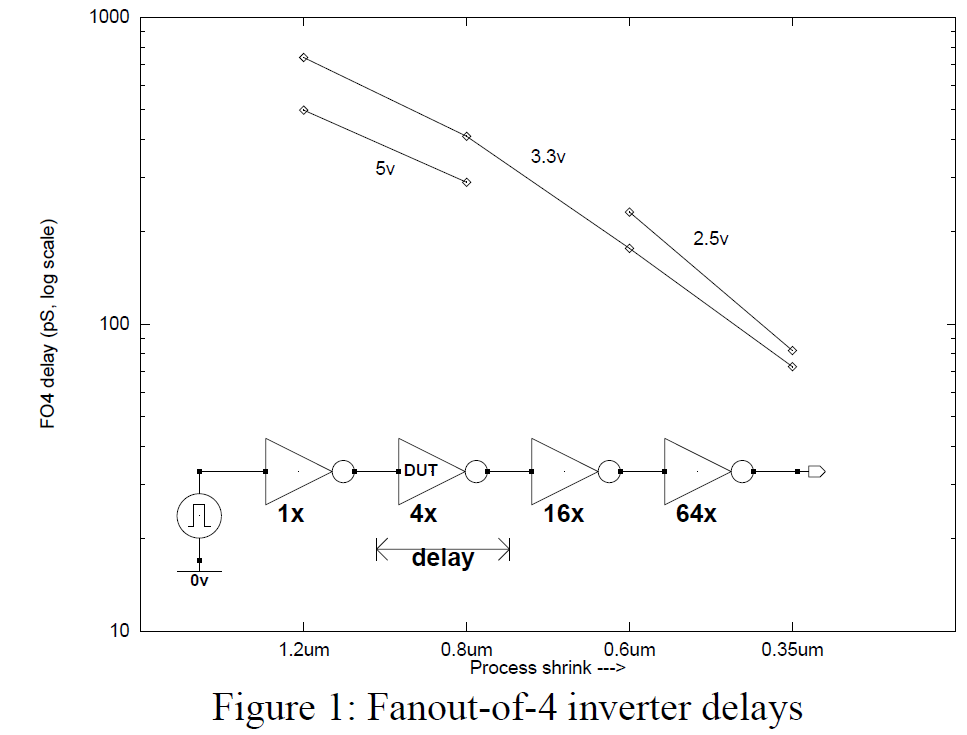
\includegraphics[height=7cm]{images/f04_figure.png}}
\end{figure}

The first inverter is designed to take the PWL/PULSE input voltage from SPICE and shape it into a realistic inverter output slope for the DUT. The inverter after the DUT provides the fanout of 4 load for the DUT. The final inverter slows the switching time of the third inverter, which prevents large Miller multiplication of the third inverter's $C_{gd}$.

I swept the width of the PMOS from 100n to 200n while performing transient simulations. I measured the propagation delays (high-to-low and low-to-high) using '.measure' statements in SPICE. Propagation delay was measured from 50\% of the input to 50\% of the output. The SPICE file is provided in the appendix. The results are summarized below:

\begin{figure}[H]
	\centerline{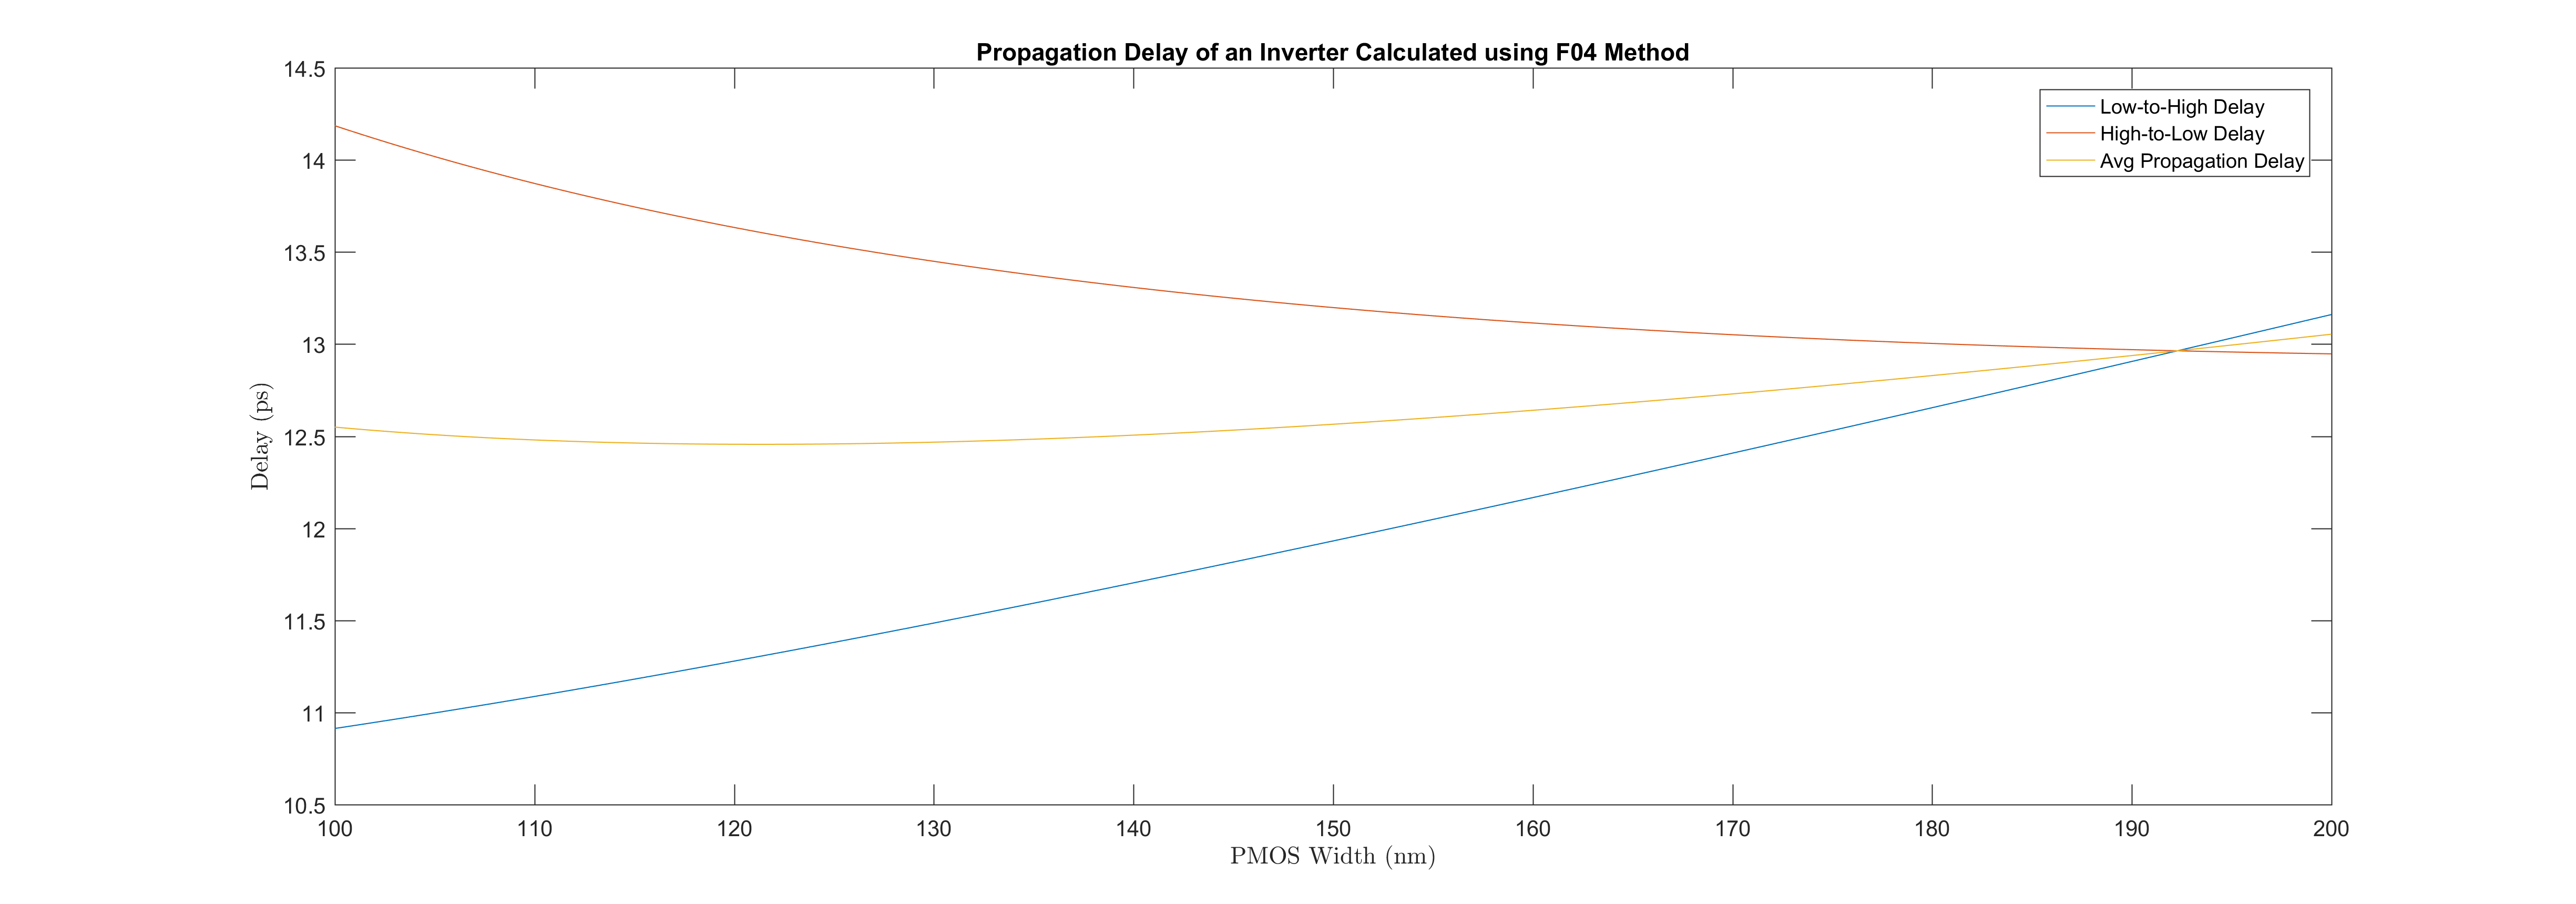
\includegraphics[height=7cm]{images/inverter_delay.png}}
\end{figure}

We find that the average propagation delay $t_p$ is minimized when the PMOS width is 121nm and the minimal delay is 12.4560 ps. The PMOS width that results in an equal low-to-high and high-to-low delay is 192.3nm and the equal delay is 12.96 ps. In conclusion, for the instructions in this part:

\begin{eqnarray}
	W_{pmos,optimal} = 121 \text{ nm for } W_{nmos} = 100 \text{ nm} \nonumber \\
	t_{p,optimal} = 12.4560 \text{ ps} \nonumber
\end{eqnarray}

\subsection{Find Optimal Inverter's Intrinsic Delay $p$}
Our next goal is to find the intrinsic delay $p$ of this optimally sized CMOS inverter. It is set 'naturally' by the ratio of diffusion to gate capacitances, but in this case we will find it using delay measurements.

We use the equation given in 151:

\begin{eqnarray}
	t_p = t_{inv} (\gamma + f) \nonumber
\end{eqnarray}

where $t_p$ is the delay through an inverter, $t_{inv}$ is a technology constant that represents the intrinsic delay of a minimum sized inverter, $\gamma$ is a process constant that describes the ratio between drain and gate capacitances, and $f$ is the fanout of the inverter. The goal is to derive $\gamma$ and $t_{inv}$ from simulations.

We use a similar setup from the previous section, except that the PMOS width is fixed at the optimal value and instead the size of the stage after the DUT is swept. The inverter before the DUT is minimally sized for input slope shaping, and the inverter after the DUT's load is 4x upsized from the variable load size.

\begin{figure}[H]
	\centerline{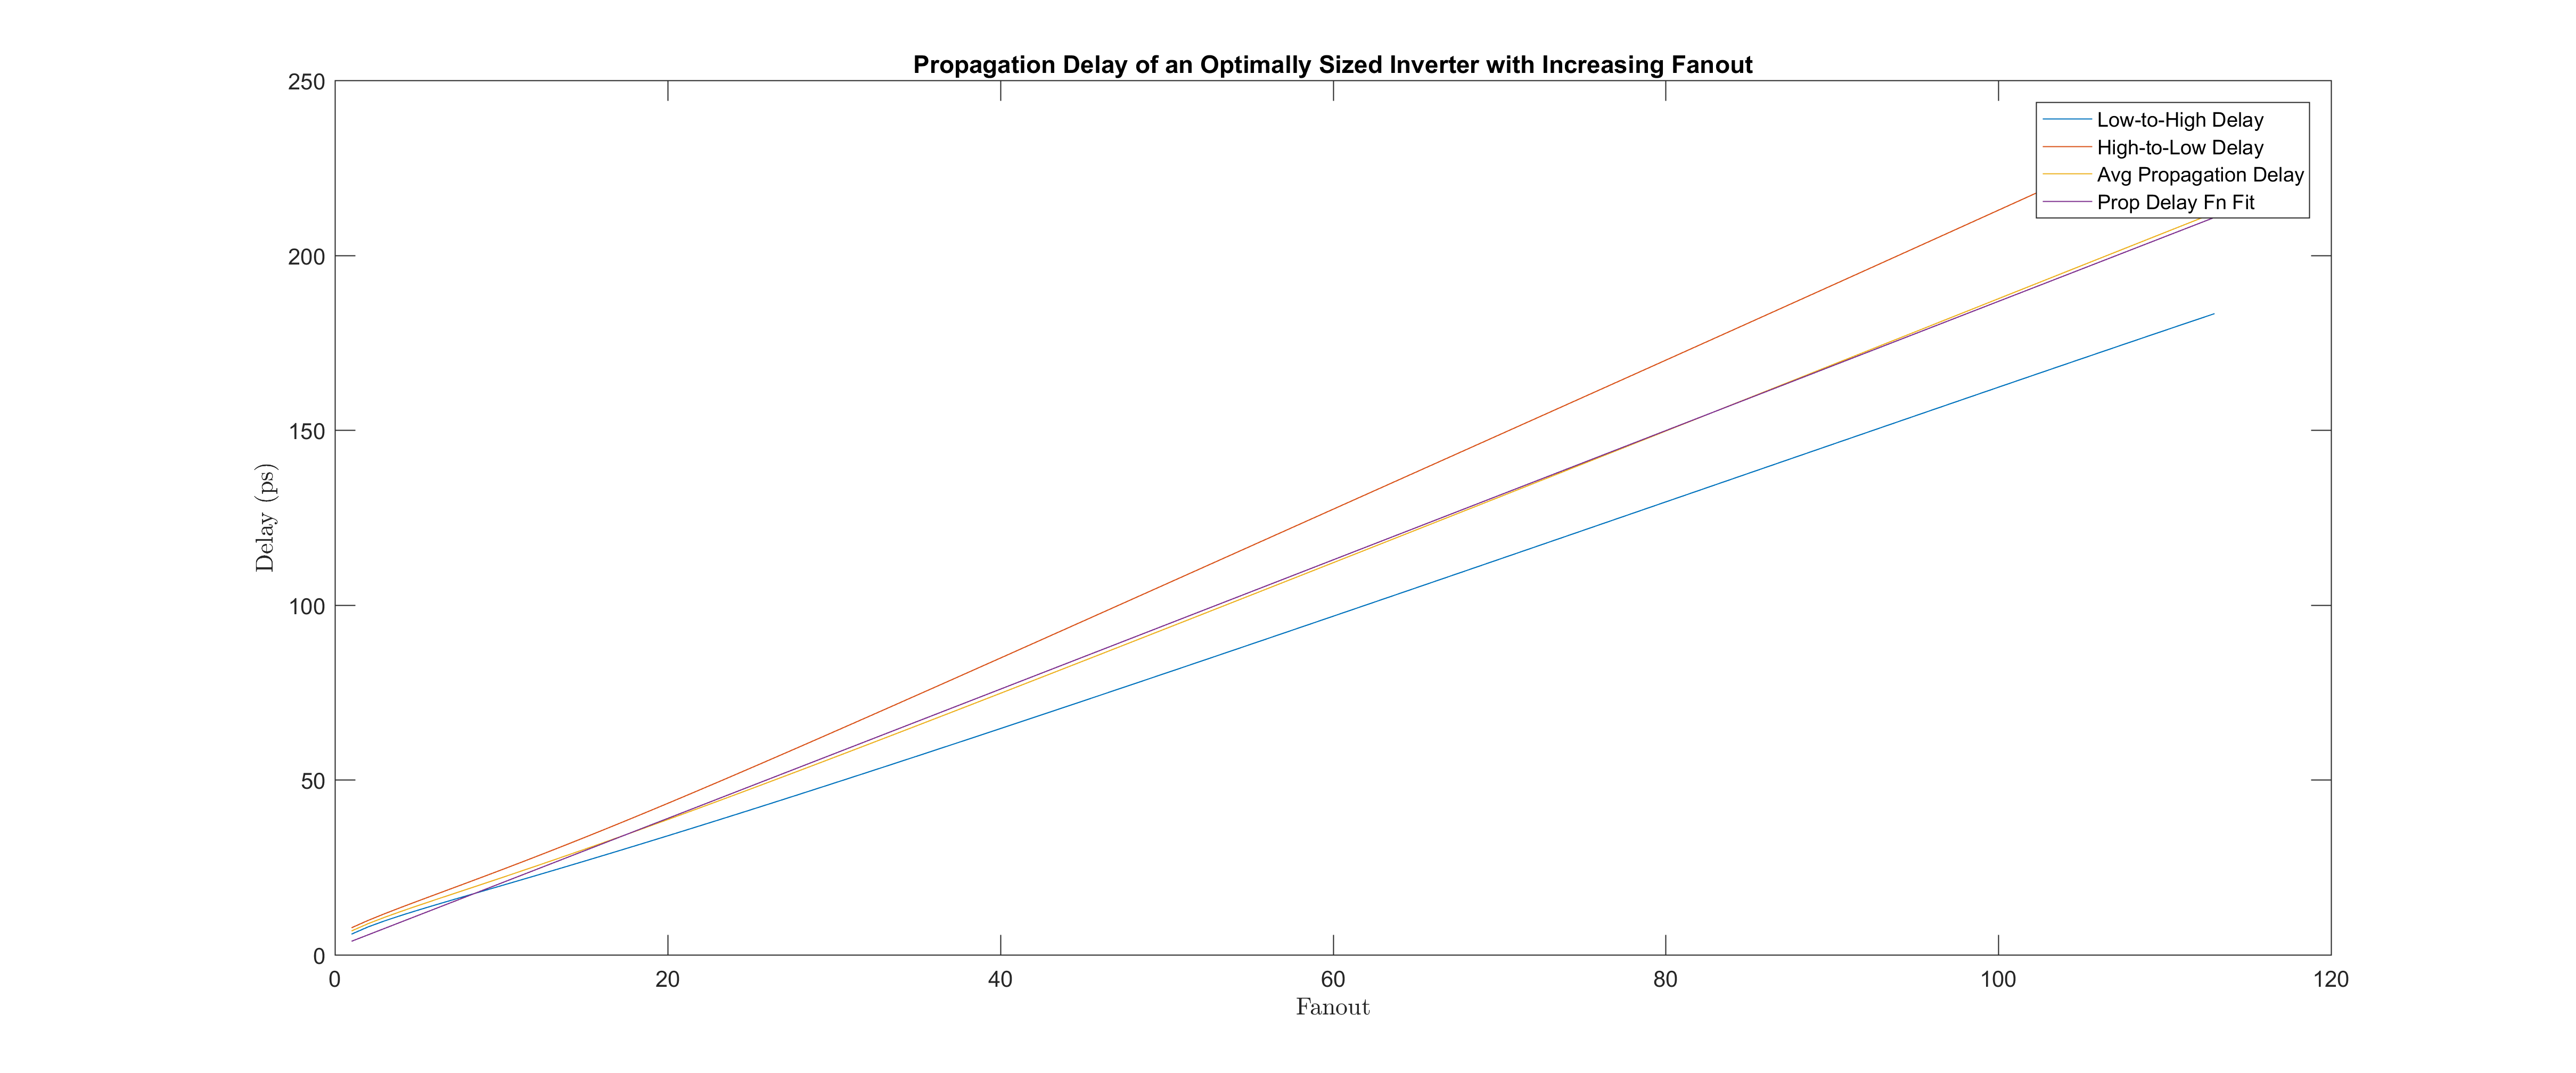
\includegraphics[width=\textwidth+2cm]{images/inverter_delay_vs_fanout.png}}
\end{figure}

We find that the best fit is given by $\gamma = 1.1011$ and $t_{inv} = 1.8478 \text{ ps}$.

\subsection{Optimal CMOS NAND2 Sizing}
We want to find the required width $W_{nmos}$ for the NMOS transistors in the pull-down network such that the equivalent resistance of the pull down network is the same as the equivalent resistance in an inverter from part a). Use hand analysis with parameters ($E_C L, V_{DD}, V_{th}$) from problem 1. We then compare the results to SPICE simulations.

We utilize the velocity saturated current model for a MOSFET and set the current of the NMOS pull-down network of the NAND2 gate equal to the current of the pull-down NMOS of the inverter for equal drive strength. We model the NAND pull-down network as 1 transistor of twice the minimum length (32nm * 2 = 64nm), and we find the optimal width.

\begin{eqnarray}
	I_{DSat} = \frac{W}{L} \frac{\mu_{eff} C_{ox} E_C L}{2} \frac{(V_{GS} - V_{th})^2}{(V_{GS} - V_{th}) + E_C L} \nonumber \\
	I_{DSat,inv} = \frac{W_{inv}}{L} \frac{\mu_{eff} C_{ox} E_C L}{2} \frac{(V_{GS} - V_{th})^2}{(V_{GS} - V_{th}) + E_C L} \nonumber \\
	I_{DSat,nand2} = \frac{W_{nand2}}{2 \cdot L} \frac{\mu_{eff} C_{ox} E_C 2 \cdot L}{2} \frac{(V_{GS} - V_{th})^2}{(V_{GS} - V_{th}) + E_C 2 \cdot L} \nonumber
\end{eqnarray}

Setting $I_{DSat,inv} = I_{DSat,nand2}$:

\begin{eqnarray}
	\frac{W_{inv}}{W_{nand2}} = \frac{(V_{GS} - V_{th}) + E_C L}{(V_{GS} - V_{th}) + 2 \cdot E_C L} \nonumber
\end{eqnarray}

We now use $V_{GS} = 1.05 \text{ V}$, $E_C L = 485.9 \text{ mV}$, and $V_{th} = 0.2039 \text{ V}$ from problem 1, and we find the width ratio. Another calculation is done using the values provided by the homework spec: $V_{GS} = 1 \text{ V}$, $E_C L = 800 \text{ mV}$, and $V_{th} = 0.5 \text{ V}$, for comparison purposes.

\begin{eqnarray}
	\frac{W_{nand2}}{W_{inv}} \text{ (my parameters)} = 1.36 \nonumber \\
	\frac{W_{nand2}}{W_{inv}} \text{ (HW given parameters)} = 1.62 \nonumber
\end{eqnarray}

To find the optimal NMOS width in SPICE for a high-to-low transition of a NAND2 gate, we use a similar setup to the F04 inverter circuit. We fix one of the inputs to the NAND2 gate at $V_{DD}$ and we let the other input rise from 0 to $V_{DD}$ to cause the gate to transition from high-to-low. We drive the switching gate input with an inverter to shape the input slope and the NAND gate's output drives 2 serially connected inverters which have a fanout of 4 each. Here's my setup; the SPICE sim file is provided in the appendix. I held the top NMOS transistor at $V_{DD}$ and I switched the bottom NMOS transistor to give the worst-case high-to-low transition.

\begin{figure}[H]
	\centerline{\includegraphics[height=3cm]{images/nmos2_setup.png}}
\end{figure}

\begin{figure}[H]
	\centerline{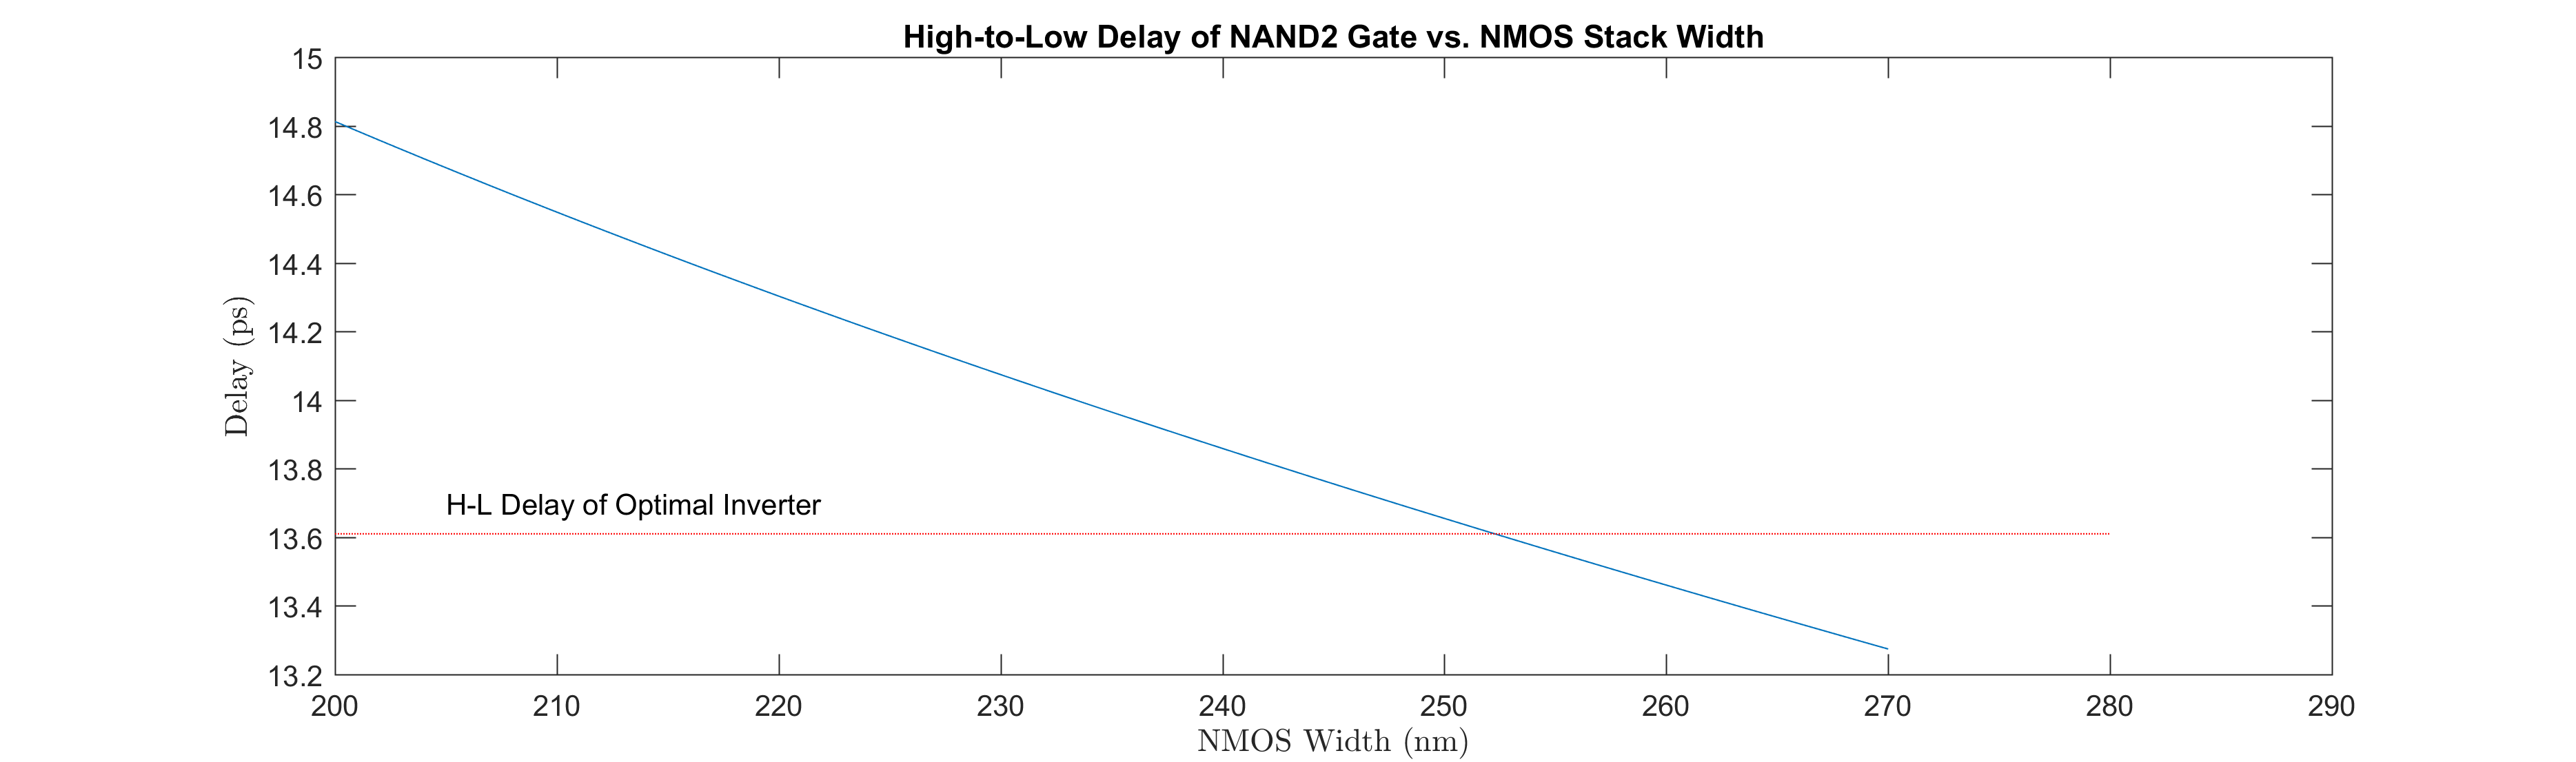
\includegraphics[height=6cm]{images/nand2_delay_vs_width.png}}
\end{figure}

We observe that the optimal NMOS width to match the pull-down strength of an inverter that's equivalently sized is significantly larger than the predicted 200nm. \textbf{The ideal width is around 252nm for the NMOS} with a 100nm width for the PMOS. This is due to the transistor stack which worsens each transistors' equivalent resistance.
 
\subsection{CMOS NAND2 Logical Effort and Intrinsic Delay}
We recall the following equation from 151:

\begin{equation*}
	t_{p,gate} = t_{inv}(p + LE \cdot f)
\end{equation*}

We want to find the intrinsic delay and logical effort of the optimally sized NAND2 gate with a high-to-low delay that matches the that of the inverter. We normalize $p$ to $p_{inv} = \gamma$, which was derived earlier. We gather data in a similar fashion by sweeping the fanout of the NAND gate and observing its delay for both low-to-high and high-to-low gate transitions. We then fit the propagation delay equation with free parameters $t_{inv}$ (the intrinsic NAND2 delay multiplied by $t_{inv}$ of an inverter) and $LE$ (the logical effort of the NAND2). Everything is normalized to the optimal, minimal inverter.

\section{5-32 Decoder Design + VLSI Flow}

\subsection{GCD: VLSI's Hello World}

Here are the first 45 lines of the post-PAR Verilog netlist:
\begin{minted}[linenos]{verilog}
module gcdGCDUnitCtrl (clk , reset_BAR , operands_val , result_rdy , 
B_zero , A_lt_B , result_val , operands_rdy , A_mux_sel , B_mux_sel , 
A_en , B_en , IN0 );
input  clk ;
input  reset_BAR ;
input  operands_val ;
input  result_rdy ;
input  B_zero ;
input  A_lt_B ;
output result_val ;
output operands_rdy ;
output [1:0] A_mux_sel ;
output B_mux_sel ;
output A_en ;
output B_en ;
input  IN0 ;


wire [1:0] state ;

AND2X1_RVT icc_clock3 (.Y ( n16 ) , .A1 ( A_lt_B ) , .A2 ( n5 ) ) ;
NBUFFX8_RVT CTSNBUFFX32_RVT_G1B3I1 (.A ( clk_G1B5I1 ) , .Y ( clk_G1B6I1 ) ) ;
INVX2_RVT CTSINVX32_RVT_G1B13I1 (.A ( clk ) , .Y ( clk_G1B1I1 ) ) ;
NBUFFX8_RVT CTSNBUFFX2_RVT_G1B1I1 (.A ( clk_G1B6I1 ) , .Y ( clk_G1B7I1 ) ) ;
NBUFFX8_RVT CTSNBUFFX2_RVT_G1B5I1 (.A ( clk_G1B2I1 ) , .Y ( clk_G1B5I1 ) ) ;
INVX16_RVT CTSINVX32_RVT_G1B11I1 (.A ( clk_G1B1I1 ) , .Y ( clk_G1B2I1 ) ) ;
INVX0_RVT icc_place4 (.A ( n7 ) , .Y ( n10 ) ) ;
DELLN1X2_RVT icc_place3 (.A ( operands_val ) , .Y ( n7 ) ) ;
DFFX1_RVT state_reg_1_ (.QN ( n17 ) , .Q ( state[1] ) , .D ( n11 ) 
, .CLK ( clk_G1B7I1 ) ) ;
NAND2X0_RVT U24 (.A2 ( n14 ) , .A1 ( n15 ) , .Y ( A_en ) ) ;
INVX0_RVT U23 (.A ( B_en ) , .Y ( n15 ) ) ;
NAND4X0_RVT U22 (.A2 ( IN0 ) , .A4 ( n8 ) , .A3 ( n9 ) , .Y ( n11 ) , .A1 ( n13 ) ) ;
INVX0_RVT U21 (.A ( result_val ) , .Y ( n8 ) ) ;
NAND2X0_RVT U20 (.A2 ( state[1] ) , .A1 ( n10 ) , .Y ( n9 ) ) ;
NAND3X0_RVT U17 (.Y ( n13 ) , .A1 ( n6 ) , .A2 ( n5 ) , .A3 ( B_zero ) ) ;
AOI21X1_RVT U16 (.Y ( n12 ) , .A2 ( n3 ) , .A3 ( reset_BAR ) , .A1 ( n4 ) ) ;
NAND2X0_RVT U15 (.A2 ( state[0] ) , .A1 ( n2 ) , .Y ( n3 ) ) ;
NAND2X0_RVT U14 (.A2 ( state[1] ) , .A1 ( result_rdy ) , .Y ( n2 ) ) ;
NAND3X0_RVT U13 (.Y ( n4 ) , .A1 ( n6 ) , .A2 ( B_zero ) , .A3 ( n17 ) ) ;
INVX0_RVT U12 (.A ( A_lt_B ) , .Y ( n6 ) ) ;
AO21X1_RVT U11 (.A1 ( operands_rdy ) , .Y ( B_en ) , .A2 ( n7 ) , .A3 ( n16 ) ) ;
NOR2X0_RVT U10 (.Y ( A_mux_sel[1] ) , .A2 ( A_lt_B ) , .A1 ( n14 ) ) ;
OR2X1_RVT U9 (.Y ( n14 ) , .A2 ( B_zero ) , .A1 ( n1 ) ) ;
INVX0_RVT U8 (.A ( n5 ) , .Y ( n1 ) ) ;
AND2X2_RVT U7 (.Y ( operands_rdy ) , .A1 ( n18 ) , .A2 ( state[1] ) ) ;
\end{minted}

\begin{enumerate}
	\item Why are you generally not worried when you have hold time violations after synthesis?
	Hold time violations can be easily resolved later in the flow by inserting dummy logic/delay or by allowing a longer wire (with greater, non-zero delay) to connect the path that has a hold time violation.
	
	\item Why does the tutorial example (page 9) fail timing even though the delay is less than the clock period (0.5ns)?
	Even though the data arrival time is below 0.5ns, the data required time is also below 0.5ns, and to a greater extend than the data arrival time. This is due to factoring in the clock uncertainty (jitter/skew introduced later in the flow), and the setup time of the flip-flop.
	
	\item Why might you want to set a conservative \verb|clock_uncertainty|?
	A conservative \verb|clock_uncertainty| will account for any clock skew and jitter added during PAR. If the \verb|clock_uncertainty| is too optimistic, you may find that timing will pass when performing post-synthesis simulation, but will fail when trying post-PAR simulation.
\end{enumerate}

\subsection{Decoder Design}

Here is my decoder implementation in \verb|decoder.v|:

\begin{minted}[tabsize=2]{verilog}
module decoder(
	input [4:0] A,
	output reg [31:0] Z,
	input clk
);
	// NOTE: Testbench expects that the output Z is registered!
	genvar i;
	generate
		for (i = 0; i <= 5'd31; i = i + 1) begin:decoder_loop
			always @ (posedge clk) begin
				Z[i] <= A == i;
			end
		end
	endgenerate
endmodule
\end{minted}

I had to modify the `timescale in the \verb|decoder_tb| to be 1ns/10ps to match the vcs invocation and to ensure that a small clock period under 100ps would simulate without issues. The behavioral simulation succeeded.

After running \verb|dc-syn|, I found that there were timing violations, and I fixed those by increasing the clock period to 0.2ns. After this, I re-ran synthesis, verified that there were no timing violations, and ran the post-synthesis VCS sim to make sure the functionality of the decoder was still in order.

I then ran \verb|icc-par| and found several timing violations after PAR. They weren't internal to the decoder block, but rather involved the decoder's \verb|Z| register driving an output load capacitance of 30fF. This load capacitance is much higher than the internal capacitances in the circuit, so it takes a longer time to drive. The register needs to drive the output cap to its proper value before the next rising edge of the clock. I found that this will take at least 0.38ns, so I modified my clock period to 0.5ns to give the tools some slack.

After running post-PAR simulation, I found I needed to further increase the clock period to 1.0ns just to fix a testbench issue where the inputs to the decoder were supplied on the falling edge of the clock, rather than just right after the rising edge Clk-to-q to more accurately simulate the actual design.

Here are the final results:

\begin{enumerate}
	\item A screenshot of the layout
	
	\begin{figure}[H]
		\centerline{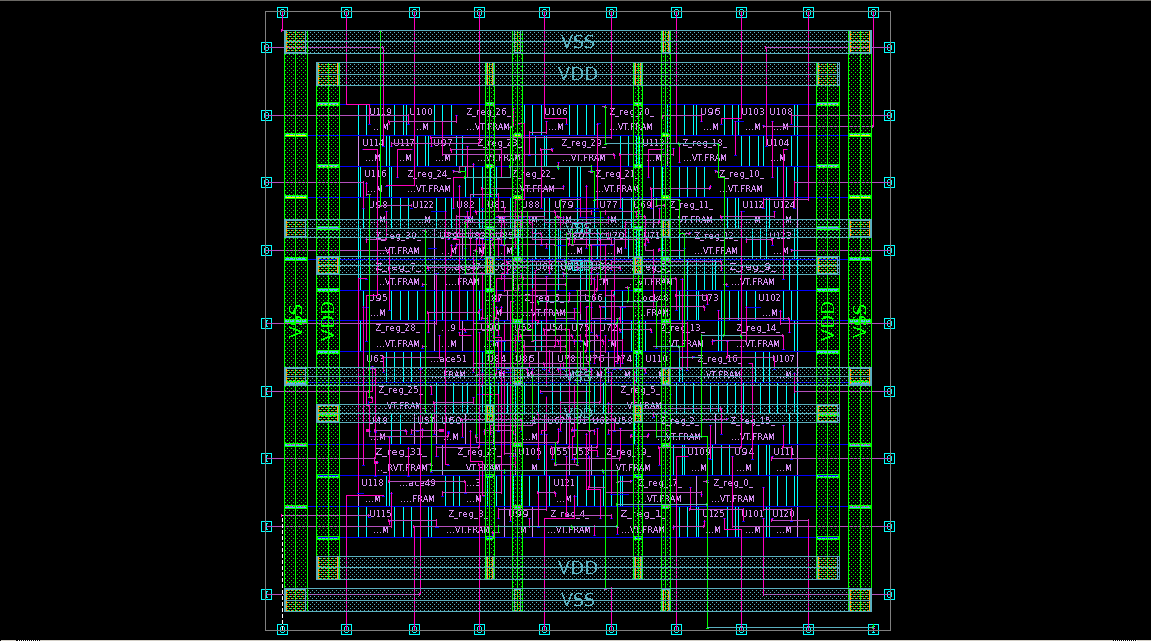
\includegraphics[width=\textwidth+2cm]{images/icc_chip_image.png}}
	\end{figure}

	\item Critical path in ns
	
	The critical path is 0.3910 ns and it starts at \verb|Z_reg_31_| and ends at \verb|Z[31]|. There is no negative slack on any path.
	
	\item Post-PAR DVE sim showing correct functionality and critical path
	
	\begin{figure}[H]
		\centerline{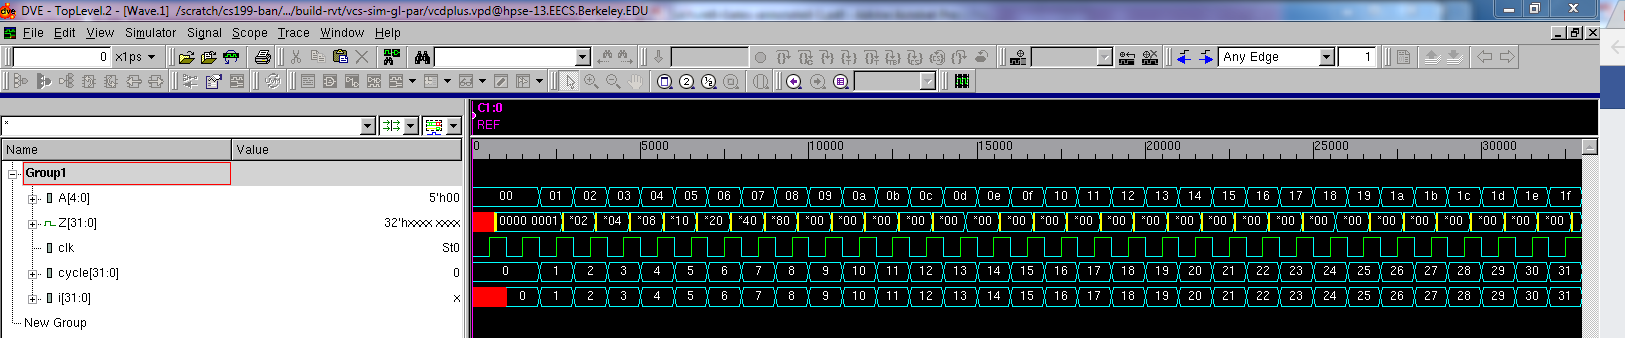
\includegraphics[width=\textwidth+2cm]{images/success_vcs_run.png}}
	\end{figure}
\end{enumerate}

\newpage
\appendix
\section{PMOS/NMOS DC Characterization SPICE Sim} \label{dc_characterization_spice}
\begin{minted}{text}
Sweep of V_GS with constant V_DS for N-MOSFET, similar file for P-MOSFET
.lib '/home/ff/ee241/synopsys-32nm/hspice/saed32nm.lib' TT
vds vds gnd 1.05
vgs vgs gnd 1.05 
x1 vds vgs gnd gnd n105 (w=1u l=32n)

.op
.dc vgs 0 1.05 10m vds 0 1.05 10m

.option post=2 nomod
.end
\end{minted}

\section{F04 Inverter PMOS Width Sweep SPICE Sim}
\begin{minted}{text}
Connecting a DUT inverter with f04 configuration

.lib '/home/ff/ee241/synopsys-32nm/hspice/saed32nm.lib' TT

* Inverter Subcircuit

.subckt inverter in out vdd gnd (pmos_width=200n, size=1)
* MOSFET instantiation: x<name> <drain> <gate> <source> <body> <model> <parameter list>
x1 out in gnd gnd n105 (w=100n*size l=32n)
x2 out in vdd vdd p105 (w=pmos_width*size l=32n)
.ends

* Test Circuit

.param pmos_width_param = 100n
vdd vdd gnd 1.05
vin vin gnd pwl(0 0 10p 0 20p 1.05 100p 1.05 110p 0)

x1 vin v1out vdd gnd inverter (pmos_width=pmos_width_param, size=1)
xdut v1out v4out vdd gnd inverter (pmos_width=pmos_width_param, size=4)
x2 v4out v16out vdd gnd inverter (pmos_width=pmos_width_param, size=16)
x3 v16out v64out vdd gnd inverter (pmos_width=pmos_width_param, size=64)

* Measurements
* We want to measure the time at which v1out has fallen to 1.05V/2
* v4out has risen to 1.05/2, v1out has risen to 1.05/2, v4out has risen to 1.05/2
.measure tran delay_l_to_h trig v(v1out) val=1.05/2 rise=1 targ v(v4out) val=1.05/2 fall=1
.measure tran delay_h_to_l trig v(v1out) val=1.05/2 fall=1 targ v(v4out) val=1.05/2 rise=1

* Analyses
.op
.tran 1f 200p START=0 SWEEP pmos_width_param 100n 200n .1n

.option post=2 nomod
.option accurate=1
.option numdgt=6
.option measdgt=6
.option delmax=10f
.end
\end{minted}

\section{F04 Inverter Delay vs Fanout SPICE Sim}
\begin{minted}{text}
Connecting a DUT inverter with f04 configuration, and sweeping fanout of its loading stage.

.lib '/home/ff/ee241/synopsys-32nm/hspice/saed32nm.lib' TT

* Inverter Subcircuit

.subckt inverter in out vdd gnd (pmos_width=121n, size=1)
* MOSFET instantiation: x<name> <drain> <gate> <source> <body> <model> <parameter list>
x1 out in gnd gnd n105 (w=100n*size l=32n)
x2 out in vdd vdd p105 (w=pmos_width*size l=32n)
.ends

* Test Circuit

* This is fixed
.param pmos_width_param = 121n
* DUT fanout
.param fanout = 4
vdd vdd gnd 1.05
vin vin gnd pwl(0 0 10p 0 20p 1.05 1n 1.05 1.01n 0)

x1 vin v1out vdd gnd inverter (pmos_width=pmos_width_param, size=1)
xdut v1out v4out vdd gnd inverter (pmos_width=pmos_width_param, size=4)
x2 v4out v16out vdd gnd inverter (pmos_width=pmos_width_param, size=4*fanout)
x3 v16out v64out vdd gnd inverter (pmos_width=pmos_width_param, size=16*fanout)

* Measurements
* We want to measure the time at which v1out has fallen to 1.05V/2
* v4out has risen to 1.05/2, v1out has risen to 1.05/2, v4out has risen to 1.05/2
.measure tran delay_l_to_h trig v(v1out) val=1.05/2 rise=1 targ v(v4out) val=1.05/2 fall=1
.measure tran delay_h_to_l trig v(v1out) val=1.05/2 fall=1 targ v(v4out) val=1.05/2 rise=1

* Analyses
.op
.tran 10p 1.2n START=0 SWEEP fanout 1 128 1

.option post=2 nomod
.option accurate=1
.option numdgt=6
.option measdgt=6
.option delmax=10f
.end
\end{minted}

\section{Decoder Post-PAR VCS Run Printout}
\begin{minted}{text}
VCD+ Writer G-2012.09_Full64 Copyright (c) 1991-2012 by Synopsys Inc.
0: A= 0, Z=xxxxxxxxxxxxxxxxxxxxxxxxxxxxxxxx, cycle=          0
1: A= 0, Z=xxxxxxxxxxxxxxxxxxxxxxxxxxxxxxx1, cycle=          0
1: A= 0, Z=x0xxxxx00x00x0xx0xx000x0xxx0x001, cycle=          0
1: A= 0, Z=x0xxx0x00x00x0xx000000x0xxx0x001, cycle=          0
1: A= 0, Z=x0xxx0x00000x000000000x0xxx0x001, cycle=          0
1: A= 0, Z=x0xxx0x00000x00000000000xx000001, cycle=          0
1: A= 0, Z=x000x0000000x0000000000000000001, cycle=          0
1: A= 0, Z=x00000000000x0000000000000000001, cycle=          0
1: A= 0, Z=x0000000000000000000000000000001, cycle=          0
1: A= 0, Z=00000000000000000000000000000001, cycle=          0
2: A= 1, Z=00000000000000000000000000000001, cycle=          1
3: A= 1, Z=00000000000000000000000000000011, cycle=          1
3: A= 1, Z=00000000000000000000000000000010, cycle=          1
3: A= 2, Z=00000000000000000000000000000010, cycle=          2
4: A= 2, Z=00000000000000000000000000000110, cycle=          2
4: A= 2, Z=00000000000000000000000000000100, cycle=          2
4: A= 3, Z=00000000000000000000000000000100, cycle=          3
5: A= 3, Z=00000000000000000000000000000000, cycle=          3
5: A= 3, Z=00000000000000000000000000001000, cycle=          3
5: A= 4, Z=00000000000000000000000000001000, cycle=          4
6: A= 4, Z=00000000000000000000000000011000, cycle=          4
6: A= 4, Z=00000000000000000000000000010000, cycle=          4
6: A= 5, Z=00000000000000000000000000010000, cycle=          5
7: A= 5, Z=00000000000000000000000000000000, cycle=          5
7: A= 5, Z=00000000000000000000000000100000, cycle=          5
7: A= 6, Z=00000000000000000000000000100000, cycle=          6
8: A= 6, Z=00000000000000000000000000000000, cycle=          6
8: A= 6, Z=00000000000000000000000001000000, cycle=          6
8: A= 7, Z=00000000000000000000000001000000, cycle=          7
9: A= 7, Z=00000000000000000000000011000000, cycle=          7
9: A= 7, Z=00000000000000000000000010000000, cycle=          7
9: A= 8, Z=00000000000000000000000010000000, cycle=          8
10: A= 8, Z=00000000000000000000000110000000, cycle=          8
10: A= 8, Z=00000000000000000000000100000000, cycle=          8
10: A= 9, Z=00000000000000000000000100000000, cycle=          9
11: A= 9, Z=00000000000000000000000000000000, cycle=          9
11: A= 9, Z=00000000000000000000001000000000, cycle=          9
11: A=10, Z=00000000000000000000001000000000, cycle=         10
12: A=10, Z=00000000000000000000011000000000, cycle=         10
12: A=10, Z=00000000000000000000010000000000, cycle=         10
12: A=11, Z=00000000000000000000010000000000, cycle=         11
13: A=11, Z=00000000000000000000110000000000, cycle=         11
13: A=11, Z=00000000000000000000100000000000, cycle=         11
13: A=12, Z=00000000000000000000100000000000, cycle=         12
14: A=12, Z=00000000000000000001100000000000, cycle=         12
14: A=12, Z=00000000000000000001000000000000, cycle=         12
14: A=13, Z=00000000000000000001000000000000, cycle=         13
15: A=13, Z=00000000000000000010000000000000, cycle=         13
15: A=14, Z=00000000000000000010000000000000, cycle=         14
16: A=14, Z=00000000000000000110000000000000, cycle=         14
16: A=14, Z=00000000000000000100000000000000, cycle=         14
16: A=15, Z=00000000000000000100000000000000, cycle=         15
17: A=15, Z=00000000000000001100000000000000, cycle=         15
17: A=15, Z=00000000000000001000000000000000, cycle=         15
17: A=16, Z=00000000000000001000000000000000, cycle=         16
18: A=16, Z=00000000000000000000000000000000, cycle=         16
18: A=16, Z=00000000000000010000000000000000, cycle=         16
18: A=17, Z=00000000000000010000000000000000, cycle=         17
19: A=17, Z=00000000000000110000000000000000, cycle=         17
19: A=17, Z=00000000000000100000000000000000, cycle=         17
19: A=18, Z=00000000000000100000000000000000, cycle=         18
20: A=18, Z=00000000000001100000000000000000, cycle=         18
20: A=18, Z=00000000000001000000000000000000, cycle=         18
20: A=19, Z=00000000000001000000000000000000, cycle=         19
21: A=19, Z=00000000000000000000000000000000, cycle=         19
21: A=19, Z=00000000000010000000000000000000, cycle=         19
21: A=20, Z=00000000000010000000000000000000, cycle=         20
22: A=20, Z=00000000000110000000000000000000, cycle=         20
22: A=20, Z=00000000000100000000000000000000, cycle=         20
22: A=21, Z=00000000000100000000000000000000, cycle=         21
23: A=21, Z=00000000001100000000000000000000, cycle=         21
23: A=21, Z=00000000001000000000000000000000, cycle=         21
23: A=22, Z=00000000001000000000000000000000, cycle=         22
24: A=22, Z=00000000000000000000000000000000, cycle=         22
24: A=22, Z=00000000010000000000000000000000, cycle=         22
24: A=23, Z=00000000010000000000000000000000, cycle=         23
25: A=23, Z=00000000110000000000000000000000, cycle=         23
25: A=23, Z=00000000100000000000000000000000, cycle=         23
25: A=24, Z=00000000100000000000000000000000, cycle=         24
26: A=24, Z=00000001000000000000000000000000, cycle=         24
26: A=25, Z=00000001000000000000000000000000, cycle=         25
27: A=25, Z=00000000000000000000000000000000, cycle=         25
27: A=25, Z=00000010000000000000000000000000, cycle=         25
27: A=26, Z=00000010000000000000000000000000, cycle=         26
28: A=26, Z=00000110000000000000000000000000, cycle=         26
28: A=26, Z=00000100000000000000000000000000, cycle=         26
28: A=27, Z=00000100000000000000000000000000, cycle=         27
29: A=27, Z=00000000000000000000000000000000, cycle=         27
29: A=27, Z=00001000000000000000000000000000, cycle=         27
29: A=28, Z=00001000000000000000000000000000, cycle=         28
30: A=28, Z=00011000000000000000000000000000, cycle=         28
30: A=28, Z=00010000000000000000000000000000, cycle=         28
30: A=29, Z=00010000000000000000000000000000, cycle=         29
31: A=29, Z=00110000000000000000000000000000, cycle=         29
31: A=29, Z=00100000000000000000000000000000, cycle=         29
31: A=30, Z=00100000000000000000000000000000, cycle=         30
32: A=30, Z=01100000000000000000000000000000, cycle=         30
32: A=30, Z=01000000000000000000000000000000, cycle=         30
32: A=31, Z=01000000000000000000000000000000, cycle=         31
33: A=31, Z=00000000000000000000000000000000, cycle=         31
33: A=31, Z=10000000000000000000000000000000, cycle=         31
**Ran through all test vectors**
$finish called from file "../../src/decoder_tb.v", line 31.
$finish at simulation time                33000
V C S   S i m u l a t i o n   R e p o r t
Time: 33000 ps
\end{minted}

\end{document}